% !TeX spellcheck = en_GB

\chapter{Modelling Neurobiological Systems}
\label{chp:modelling_neurobiological_systems}

\begin{OpeningQuote}
First, it is an overstatement to describe what I am attempting here as an \enquote{approach toward the understanding}; it is merely a somewhat systematized set of speculations as to how such an approach ought to be made. That is, I am trying to guess which of the---mathematically guided---lines of attack seem, from the hazy distance in which we see most of them, a priori promising, and which ones have the opposite appearance.
\OpeningQuoteSource{John von Neumann}{The Computer and the Brain (1958)}
\end{OpeningQuote}

\begin{PriorPublication}
Parts of this chapter, particularly \Cref{sec:nef}, are based on \citet{stoeckel2021}.
Some figures in this chapter were adapted from material previously prepared for the University of Waterloo course SYDE 556/720, \enquote{Simulating Neurobiological Systems} taught by the author in winter 2020.
\end{PriorPublication}

% !TeX spellcheck = en_GB

The desire to understand cognition is by no means a new one---wondering about one's own thought processes has surely been part of the human condition since prehistoric times.
Today, we know that nerve cells in the brain are the primary functional and structural units that give rise to biological cognition.
This is referred to as the \emph{neuron doctrine}, a view that garnered support through observations made by Santiago Ramón y Cajal and Charles Scott Sherrington at the turn of the nineteenth century \citep[Chapter~2]{yuste2015neuron,bear2016neuroscience}.

Although the nature of neurons as independent units is undisputed, the neuron doctrine continues to be scrutinised.
There is an argument to be made that neural circuits are better described from the perspective of neural ensembles instead of individual neurons \citep{yuste2015neuron,churchland1992computational}---an idea that we revisit in the context of population codes.
Furthermore, it is still a matter of debate in how far structures such as Glial cells, must be taken into account to accurately model brain function \citep[e.g.,][]{verkhratsky2000ion}.

\begin{figure}
	\centering
	\includegraphics{media/chapters/02_modelling/02_00/levels.pdf}
	\caption[Illustration of temporal and spatial scales in neuroscience]{Illustration of temporal and spatial scales in neuroscience. Placement of individual concepts is deliberately coarse and, in some cases, open to debate. Spatial scale and levels of organisation adapted from \citet[Figure~1.4, p.~11]{churchland1992computational}.
	Temporal scales inspired by \citet[Figure~1]{sejnowski2014putting}.
	}
	\label{fig:spatial_and_temporal_scales}
	\vspace*{-0.5em}
\end{figure}

The fact that,  after more than a century of research, such fundamental debates still persist, illustrates that neuroscience (and by extension the other cognitive sciences) are still in their early days.
This is not due to a lack of talent or dedication;
rather, the gaps in our knowledge are a testament to the intrinsic difficulty of understanding complex systems such as the brain.

In some regard, neuroscience may be compared to physics.
Both fields study and predict the behaviour of natural systems, and both study phenomena that span vast spatial and temporal scales
(cf.~\Cref{fig:spatial_and_temporal_scales}).
Unlike physics, neuroscience is concerned with the behaviour of living objects consisting of billions of complex elements.%
\footnote{The human brain has $67$-$86\times10^{9}$ neurons and $\sim$$85\times10^9$ glial cells \citep{vonbartheld2016search}. Each neuron in cerebral cortex possesses $10^3$-$10^4$ synapses \citep[Chapter~6]{braitenberg2013anatomy}.}
The evolved nature of brains in particular makes it challenging to disentangle structures merely responsible for metabolic function, from those orchestrating behaviour.
Therefore, as demanded by many in the field \citep[e.g.,][]{marr1982vision,churchland1992computational,eliasmith2003neural}, neuroscience should be guided by predictive computational modelling and theory.%, with the goal to systematically connect mechanisms to behaviour, and to abstract unnecessary detail.

Here, the term \enquote{theory}, refers to overarching concepts applicable to different models \citep[e.g.,][]{stevens2000models}.
Continuing our physics analogy, successful physical theories such as Newtonian or Lagrangian mechanics, describe phenomena at different scales---from falling apples to solar systems orbiting their galactic centre.
Translating this to neuroscience, we would like our theories to connect low-level mechanisms (e.g., neurons, synapses, action potentials) to high-level behaviour (e.g.,~motor control, decision making, language).
As of now, there is no widely accepted theory that accomplishes this \citep[Chapter~9]{eliasmith2013how}.

All this is not to say that neuroscience has stagnated over the past decades.
To the contrary.
New recording methods---such as fMRI (functional magnetic resonance imaging), high-density multi-electrode arrays, calcium imaging, and optogenetics---have widened our perspective on brain function \citep{sejnowski2014putting}. Researchers have mapped out individual brain circuits \citep[e.g.,][]{shepherd2012handbook}, can describe neurons at a molecular level \citep[e.g.,][]{sobolevsky2009xray}, and determined the roles specific brain regions play in cognition \citep[e.g.,][]{kanwisher2006fusiform}.

Paradoxically, recent progress in neuroscience has made finding theories that bridge multiple levels of analysis \emph{more}, and not less important.
The central challenge is that each dataset on its own is fairly limited, mostly because different recording techniques possess dissimilar temporal and spatial characteristics \citep{sejnowski2014putting}.
The data we have access to is not detailed enough to directly inform large-scale models, and our theories are not sophisticated enough to combine heterogneous datasets. As pointed out by \citet{churchland1992computational}, there is an argument to be made that neuroscience has been, and still is, \enquote{data poor \emph{and} theory poor}.
A major difficulty in modelling brain function hence lies in building models that can be constrained by, and that make predictions compatible with, the different scales at which current recording techniques operate \citep[Chapter~9]{eliasmith2013how}.

As of now, there are a few attempts at developing such theories, or, less ostentatiously, \emph{modelling frameworks}, that facilitate describing the nervous systems at different scales.
Examples include the Neural Engineering Framework (\NEF; \cite{eliasmith2003neural}), Efficient, Balanced Spiking Networks (\EBN; \cite{boerlin2011spikebased,boerlin2013predictive}), and, to some degree, FORCE~\citep{sussillo2009generating,nicola2017supervised}.
Generally speaking, these approaches describe how to translate dynamical systems---corresponding to some hypothesized behavioral model---into an idealized spiking neural network that adheres to desired neurophysiological constraints.
Depending on the specific method, this can include neural tuning, firing rate distributions, and population-level connectivity~\citep{komer2016unified,nicola2017supervised}.
The resulting networks can then be analysed using the same techniques as biological systems, bridging the gap between empirical data and theory.

As we mentioned in \Cref{chp:introduction}, a goal of this thesis is to extend the Neural Engineering Framework to better take mechanistic constraints often found in the neuroscience literature into account.
To this end, we first review fundamental neuroscientific concepts, and then describe the \NEF along with list of biological constraints currently not well-captured by the \NEF.
We then, in subsequent chapters, propose extensions to the \NEF that, to some degree, alleviate these issues.
Finally, we demonstrate constructing a detailed biological of eyeblink conditioning in the cerebellum.


\clearpage
\setcounter{section}{0}
% !TeX spellcheck = en_GB

\section{Morphology and Physiology of Individual Neurons}
\label{sec:neurophysiology}

\begin{figure}
	\centering
	{\phantomsubcaption\label{fig:neuron_sketches_motor}}%
	{\phantomsubcaption\label{fig:neuron_sketches_pyramidal}}%
	{\phantomsubcaption\label{fig:neuron_sketches_purkinje}}%
	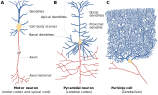
\includegraphics{media/chapters/02_modelling/02_01/neuron_sketches.pdf}
	\caption[Drawings of neurons in different brain regions]{Drawings of neurons in different brain regions.
	Although key structural elements can be identified across neurons, they can have very different morphologies.
	Redrawn from Ramón y Cajal.
	Overall presentation from \citet{kandel2012principles}, Figure~2-3D, p.~25.
	\textbf{(A)} Schematic drawing of a motor neuron (\cite{ramonycajal1894nouvelles}, Figure 6, p.~25).
	\textbf{(B)} Human cortical pyramidal neuron (\cite{howell1916textbook}, Figure~84, p.~187).
	\textbf{(C)} Human purkinje cell in the cerebellum (\cite{ramonycajal1909histologie}, Figure~9, p.~61).
	\label{fig:neuron_sketches}
	}
\end{figure}

Neurons come in various sizes, shapes, and degrees of interconnectedness.
Ramón y Cajal's\index{Ramón y Cajal, Santiago} drawings (schematically redrawn in \Cref{fig:neuron_sketches}) offer a glimpse of the morphological diversity found in the nervous system.
Some neurons possess only few branches (also \emph{projections}\index{neuron!projection}) and have a comparably simple structure, whereas others, such as Cerebellar Purkinje cells, feature sprawling dendritic trees more deserving of the name \enquote{dendritic forest}.

It should come as no surprise that the following review of neural morphology and physiology cannot do justice to the incredible complexity observed in nature.
Our goal is to instead focus on structural and functional elements commonly observed across all neurons.
As a side-effect, the resulting characterisation of the nervous system lends itself well to computational models.
%While the simplifications we make come at the risk of ignoring details that could turn out to be essential for modelling brain function, some simplification
%Yet, as discussed above, we would like to develop theories that bridge as many levels of scale as possible.
%The aspects of biology that we incorporate into our models are known to play a major role in overall brain function.
We open with a high-level overview of neural function and structure, and then focus on aspects of neural electrophysiology that will be relevant in later sections, including the generation of the membrane potential, action potentials, and synaptic transmission.
Readers interested in a more thorough introduction to neuroscience are encouraged to consult neuroscience textbooks such as \citet{bear2016neuroscience}, \citet{purves2017neuroscience}, or \citet{kandel2012principles}.

\subsection{Functional and Structural Overview}
\label{sec:neurons_overview}

\begin{figure}
	\centering
	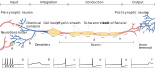
\includegraphics{media/chapters/02_modelling/02_01/neuron_signals_overview.pdf}
	\caption[Overview of neural function]{Overview of neural function. Inset diagrams illustrate the membrane potential over time at the indicated locations (data from a compartmental Hodgkin-Huxley-type model neuron). Arrows indicate the predominant flow of information. \emph{Input:} Neurons receive signals from pre-synaptic neurons through synapses. For chemical synapses, action potentials (\enquote{spikes}) arriving at the synapse (\emph{a}) cause a release of neurotransmitter that induces a post-synaptic potential (PSP) in the post-synaptic neuron (\emph{b}). \emph{Integration:} PSPs from multiple pre-synaptic neurons interact in the dendrites. Under certain conditions the neuron produces its own action potential (\emph{c}). \emph{Conduction:} The action potential travels along the axon (\emph{d}-\emph{e}). \emph{Output:} The neuron induces a PSP in a post-synaptic neuron (\emph{f}).
	}
	\label{fig:neuron_signal_overview}
\end{figure}

From the perspective of computer science---and as suggested by the neuron doctrine---neurons are fundamental units of computation in biological systems.
Specifically, neurons employ weak bioelectric signals, variations in their membrane potential, to compute.
As depicted in the lower portion of \Cref{fig:neuron_signal_overview}, these variations can either be gradual, as is the case when the neuron is in its \emph{subthreshold} regime\index{membrane potential!subthreshold}, or manifest themselves as rapid swings between the highest and lowest voltages that can be produced by a neuron; in this case the neuron is in its \emph{superthreshold} regime.
These rapid voltage changes are called \emph{action potentials}\index{action potential}, or, more colloquially, \enquote{\emph{spikes}}, harking back to their prominent appearance on oscillograms.
% TODO: Index: spike -> action potential

Typically, gradual subthreshold potentials are not directly accessible from other parts of the network;
this analogue code is solely part of a neuron's internal state.
Hence, from the perspective of other neurons in the network, a neuron is either \enquote{silent} or \enquote{spiking}.
This binary nature of neurons fascinated early computer scientists such as \citet{vonneumann1958computer}\index{Von Neumann,John} and led to the development of the first artificial neural networks by \citet{mcculloch1943logical}.

Neuroscientists typically divide neural information processing into four stages: input, integration, conduction, and output \citep[Chapter 2]{kandel2012principles}.
These stages roughly correspond to different features of neural structure, as depicted in \Cref{fig:neuron_signal_overview}.

The \emph{input region} corresponds to the dendrites, and the synapses embedded therein.%
\footnote{
The difference between input and output regions of a neuron is not always clear-cut.
Invertebrate unipolar cells only possess a single branch that protrudes from the cell body.
This branch is referred to as \enquote{axon} although it carries both input and output \citep[Chapter~2]{kandel2012principles}.}
Dendrites are tree-like structures protruding out of the cell body, typically less than two millimetres long \citep[Chapter~1]{bear2016neuroscience}.
They are usually classified according to their location relative to the cell body.
For example, in pyramidal cells (cf.~\Cref{fig:neuron_sketches_pyramidal}) dendrites directly connected to the soma are called \emph{basal}\index{dendrite!basal^}; dendrites indirectly connected to the soma through longer projections are called \emph{apical}\index{dendrite!apical}.
Apical dendrites are sometimes additionally divided---using standard anatomical terminology---into parts referred to as \emph{proxmial} or \emph{distal}; that is, they are either closer or father away from the soma \citep[e.g.,][Figure~5]{seamans1997contributions}.

Synapses form the coupling sites between neurons and---in the case of chemical synapses discussed below---establish a unidirectional flow of information.
This ensures that pre-synaptic neurons only influence the state of the post-synaptic neuron, but not vice-versa \citep[Chapter~8]{kandel2012principles}.
Some neurons in the periphery of the nervous system act as sensors; they transduce modalities such as temperature, pressure or light and do not rely on synaptic inputs \citep[Chapter~22]{kandel2012principles}.

The neuron's \emph{integration region} is formed by the cell body and, to some degree, the dendritic tree itself.
Signals from several pre-synaptic neurons interact here.
This interaction may elicit the generation of an output signal.
As we mentioned before, this output takes the form of an \emph{action potential}\index{action potential} in most vertebrate neurons \citep[Chapter~2]{kandel2012principles}.
Crucially, and in contrast to artificial neural networks, the integration process has a temporal component; the input \emph{history} is relevant for the generation of the output, and not just the momentary input.

The \emph{conductive region} corresponds to a neuron's axon\index{axon}.
The axon carries signals generated by the neuron to other parts of the nervous system.
Two features of the axon work in tandem to ensure signal integrity \citep[Chapter~7]{kandel2012principles}.
First, the axon is electrically well insulated, being tightly wrapped in Schwann's cells\index{Schwann's cell}, a type of glial cell\index{glial cell}.
Second, axons actively renew action potentials at Nodes of Ranvier\index{Node of Ranvier}, gaps between neighbouring Schwann's cells.
Conduction is unidirectional in the sense that action potentials only travel away from the origin of excitation.
Notably, in larger animals such as humans, individual neurons conduct signals across micrometres (between neighbouring neurons), centimetres (connecting different parts of the brain), and metres (motor neurons in the spinal cord).%

Finally, the \emph{output region} corresponds to the area surrounding the synapses that lie between the axon terminals and post-synaptic dendrites.
In the case of chemical synapses, the arrival of an action potential at the axon terminal causes the release of neurotransmitter molecules.
Receptors in the post-synaptic neuron transduce neurotransmitters into an input signal, a post-synaptic potential.
In the periphery, axon terminals may be coupled to muscle fibres, where the arrival of an action potential generates movement \citep[Chapter~8~\&~9]{kandel2012principles}.

\subsection{Ion channels and the membrane potential}
\label{sec:membrane_potential}

\begin{figure}
	\centering
	{\phantomsubcaption\label{fig:neuron_membrane_potential_membrane}}%
	{\phantomsubcaption\label{fig:neuron_membrane_potential_membrane_isolated}}%
	{\phantomsubcaption\label{fig:neuron_membrane_potential_membrane_channel}}%
	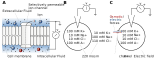
\includegraphics{media/chapters/02_modelling/02_01/neuron_membrane_potential.pdf}
	\caption[Membrane potential as a result of selectively permeable ion channels]{
	Membrane potential as a result of selectively permeable ion channels.
	\textbf{(A)} The cell membrane separates the intra- and extracellular fluid. Charge carriers (e.g., ions) are in solution in the fluids. The membrane potential is the voltage \vMem across the membrane.
	Specific ions may pass through selectively permeable channels.
	\textbf{(B)} If the membrane was a perfect insulator, there would be no membrane potential. Molar concentration in $\mathrm{mM} = \si{\milli\mole\per\litre}$; values illustrative. $A^-$ corresponds to charged anionic molecules.
	The individual fluids are electrically neutral.
	\textbf{(C)} Adding a selectively permeable ion channel results in a membrane potential specific to the ion species at which electric and osmotic forces cancel out.
	Illustrations (B, C) adapted from \citet{reichert2000neurobiologie}, Figures 2.8 and 2.10.}
\end{figure}

As mentioned above, neurons process information by systematically varying their membrane potential\index{membrane potential}\index{potential!membrane} \vMem (more precisely, their \emph{transmembrane} potential).
The membrane potential is the electrical potential between the inside and outside of a cell.
The boundary between these regions is formed by the cell membrane, a double-layer of lipids.%
\footnote{To be clear, \emph{all} biological cells possess bioelectrical properties, including a membrane potential.
This was for example analysed in detail by Julius Bernstein\index{Bernstein, Julius} in the early 1900s \citep{bernstein1912elektrobiologie}. Membrane potentials are important for homeostasis and cell-to-cell communication \citep{moorhouse2016membrane}.
For example, electrical gradients between cells are crucial for laying out the body plan of organisms \citep{levin2014molecular}.
Neurons should be thought of as cells shaped by evolution to excel at bioelectrical signalling, but are not unique in their use of bioelectricity.}
By convention, if the \emph{inside} is more positively charged than the outside, we report a positive voltage (\Cref{fig:neuron_membrane_potential_membrane}).

Measuring the membrane potential when a neuron is at rest---that is, when the cell does not receive any input---reveals the so-called resting potential \vRest.
In mammals, \vRest ranges from \SIrange{-50}{-85}{\milli\volt} depending on the cell type \citep{moorhouse2016membrane}.

Upon closer investigation, the presence of a non-zero resting potential is rather surprising.
The inside and outside of the cell are filled with watery solutions: the intracellular fluid (\enquote{cytoplasm}\index{cytoplasm}) and the extracellular fluid.
Both fluids are electrically neutral.
That is, although the fluids contain ions and anionic charge carriers in solution, the overall positive and negative charges are balanced.
There should be no measurable electrical potential (\Cref{fig:neuron_membrane_potential_membrane_isolated}).


\subsubsection{Selectively permeable ion channels generate the membrane potential}
\begin{figure}
	\centering
	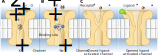
\includegraphics{media/chapters/02_modelling/02_01/channel.pdf}%
	{\phantomsubcaption\label{fig:ion_channels_k}}%
	{\phantomsubcaption\label{fig:ion_channels_na}}%
	{\phantomsubcaption\label{fig:ion_channels_gate}}%
	\caption[Schematic illustration of ion channels  embedded into the cell membrane]{Schematic illustration of ion channels embedded in the cell membrane. Ion channels are pores that selectively let ions of a certain species pass. Selectivity is achieved by exploiting the radius and charge distributions of the ion and its watery hull. \textbf{(A)} Although the $\mathrm{K^+}$ ion is larger than the $\mathrm{Na^+}$ ion, its watery hull is more compact, and it can pass through narrower channels. \textbf{(B)}  $\mathrm{Na^+}$ selectivity is achieved by a negative binding site in the channel that stabilises the $\mathrm{K^+}$ ion and its hull to let it pass.  \textbf{(C)} Ion channels can change their conformation depending on external factors (e.g.~mechanical forces, chemicals, electrical potentials); here, a chemical ligand opens a channel. Inspired by \citet[Figure~5-1, p.~102 and Figure~5-6, p.~109]{kandel2012principles}; see ibid.~for more information.}
\end{figure}
The resting potential can be explained if we assume that the cell membrane is selectively permeable to some ions through so-called \emph{ion channels}\index{ion channel}.
The presence of ion channels has been postulated for a long time, though it is only thanks to relatively recent studies that we understand the molecular machinery that underpins selective permeability \citep[Chapter~5]{kandel2012principles}.

Ion channels are porous proteins embedded in the cell membrane.
They accomplish the impressive feat of acting as an \enquote{atomic sieve}.
This \enquote{sieve} only lets a single ion of a certain kind (in chemical parlance: \emph{ion species}\index{ion species}) pass at a time, as is illustrated in \Cref{fig:ion_channels_k,fig:ion_channels_na}.
Furthermore, as we will see both in the context of action potential generation and synaptic transmission, these proteins can change their shape, or \emph{conformation}, depending on various external circumstances, effectively opening or closing the channel (\Cref{fig:ion_channels_gate}).

Of course, the mere presence of selectively permeable channels does not explain the membrane potential.
For this, we have to consider that despite being electrically neutral, the intra- and extracellular fluids contain different concentrations of the individual charge carriers.
In particular, there are large concentration gradients for potassium ($\mathrm{K^+}$), sodium ($\mathrm{Na^+}$) and chloride ($\mathrm{Cl^-}$) ions.
For example, the concentration of potassium ions $\mathrm{K^+}$ is about \SI{140}{\milli\mol\per\litre} in the cytoplasm, compared to \SI{3}{\milli\mol\per\litre} in the extracellular fluid.
If the cell membrane was permeable to $\mathrm{K}^+$ ions, an osmotic force would act on the ions, driving them outside.

This ionic flow disturbs the charge balance of the intra- and extracellular fluids and results in a non-zero membrane potential.
In turn, this potential results in an electric force that counters the osmotic pressure.
In our $\mathrm{K}^+$ example, the intracellular fluid becomes negatively charged and the ensuing electric attraction reduces the net force acting on the $\mathrm{K}^+$ ions.
The system converges to an equilibrium point where the electric and osmotic forces cancel out (\Cref{fig:neuron_membrane_potential_membrane_channel}).
The membrane potential at this point is called the \emph{equilibrium}\index{equilibrium potential}\index{potential!equilibrium} or \emph{reversal potential}\index{reversal potential}\index{potential!reversal}, as the ionic flow direction reverses at this point.
For clarity, we use the term reversal potential when talking about the equilibrium potential for a membrane permeable to a \emph{single} ion.


\subsubsection{A single selectively permeable ion channel: The Nernst equation}
For a single charge carrier $X$, the reversal potential $E_X$ can be computed using the Nernst equation\index{Nernst equation} \citep{nernst1888kinetik}:%
\footnote{The Nernst equation was published in 1888, before there were established theories about bioelectricity. Nernst studied the electrochemistry of electrolytes separated by membranes and this research was later incorporated into analyses of biological cell membranes by Ostwald and later Bernstein \citep[see][Chapter~5]{bernstein1912elektrobiologie}\index{Bernstein, Julius}.}
\newcommand{\Cout}[1]{\ensuremath{[\mathrm{#1}]_\mathrm{out}}}
\newcommand{\Cin}[1]{\ensuremath{[\mathrm{#1}]_\mathrm{in}}}
\begin{align}
	E_X &= -\frac{RT}{zF} \log \left( \frac{\Cin{X}}{\Cout{X}} \right) \,,
	\label{eqn:nernst}
\end{align}
where $R$ is the gas constant, $T$ is the temperature, $z$ is the charge number, or valence\index{valence}, of the particle (e.g., $z = 2$ for $\mathrm{Ca}^{2+}$ and $-1$ for $\mathrm{Cl}^-$) and $F$ is the Faraday constant. \Cout{X} and \Cin{X} are the concentrations (count per volume) of particles $X$ outside and inside the cell, respectively.
Note that the number of ions flowing through the cell membrane is rather minuscule compared to the total number of ions in solution; \Cout{X} and \Cin{X} essentially do not change over time.%
\footnote{The ion concentrations in the intra- and extracellular fluid are maintained by ion pumps in the cell membrane. These pumps are secondary for a cell's short-term bioelectrical properties, but are indispensible in the long run.}

\begin{table}
	\centering
	\caption[Ion concentrations and reversal potentials in the squid and mammals]{Ion concentrations and reversal potentials in the squid and mammals. Data from \citet[Table~12.1, p.~353]{mccormick2014membrane}. The squid data are based on \citet{hodgkin1949effect}, and reported similarly in \citet[Table~6-1, p.~128]{kandel2012principles}. Reversal potentials computed using \cref{eqn:nernst}.}
	\label{tbl:nernst}
	\small
	\sffamily
	\begin{tabular}{l l p{0.25cm} r r p{0.25cm} r r}
		\toprule
		&
		&
		& \multicolumn{2}{c}{\textbf{Concentrations}}
		&
		& \multicolumn{2}{c}{\textbf{Reversal potentials}} \\ %  \multicolumn{1}{c}{\textbf{Permeability ratios}}\\
		\cmidrule(lr){4-5}\cmidrule(lr){7-8}
		
		\multicolumn{2}{l}{\textbf{Ion species}}
		&
		& \emph{Intracellular}
		& \emph{Extracellular}
		&
		& $T = \SI{20}{\degreeCelsius}$
		& $T = \SI{36}{\degreeCelsius}$ \\ %& $P_\mathrm{K^+} : P_\mathrm{Na^+} : P_\mathrm{Cl^-}$ \\
		\midrule

		\multicolumn{2}{l}{\emph{Squid giant axon}}\\

		\raggedleft \quad Potassium
		& $\mathrm{K}^+$
		&
		& \SI{400}{\milli\mol\per\litre}
		& \SI{20}{\milli\mol\per\litre}
		&
		& \SI{-76}{\milli\volt}
		& \SI{-80}{\milli\volt} \\

		\raggedleft \quad Sodium
		& $\mathrm{Na}^+$
		&
		& \SI{50}{\milli\mol\per\litre}
		& \SI{440}{\milli\mol\per\litre}
		&
		& \SI{55}{\milli\volt}
		& \SI{58}{\milli\volt} \\

		\raggedleft \quad Chloride
		& $\mathrm{Cl}^-$
		&
		& \SI{40}{\milli\mol\per\litre}
		& \SI{560}{\milli\mol\per\litre}
		&
		& \SI{-67}{\milli\volt}
		& \SI{-70}{\milli\volt} \\[0.25cm]

		\multicolumn{2}{l}{\emph{Mammalian neuron}}\\

		\raggedleft \quad Potassium
		& $\mathrm{K}^+$
		&
		& \SI{140}{\milli\mol\per\litre}
		& \SI{3}{\milli\mol\per\litre}
		&
		& \SI{-97}{\milli\volt}
		& \SI{-102}{\milli\volt} \\

		\raggedleft \quad Sodium
		& $\mathrm{Na}^+$
		&
		& \SI{18}{\milli\mol\per\litre}
		& \SI{145}{\milli\mol\per\litre}
		&
		& \SI{53}{\milli\volt}
		& \SI{56}{\milli\volt} \\

		\raggedleft \quad Chloride
		& $\mathrm{Cl}^-$
		&
		& \SI{7}{\milli\mol\per\litre}
		& \SI{120}{\milli\mol\per\litre}
		&
		& \SI{-72}{\milli\volt}
		& \SI{-76}{\milli\volt} \\

		\bottomrule
	\end{tabular}
\end{table}

\subsubsection{Multiple selectively permeable ion channels: The Goldman-Huxley-Katz equation}
\Cref{tbl:nernst} lists the ion concentrations of the squid giant axon---a model system common in the early days of neuroscience---as well as mammalian cells.
Although there are large differences in the ion concentrations, the reversal potentials (when computed using eq.~\ref{eqn:nernst}) are similar across species.
Still, we find that, in general, no individual reversal potential exactly matches the resting potential.
For example, in the squid, the resting potential is close to \SI{-62}{\milli\volt} at a temperature of \SI{20}{\degreeCelsius} (\cite{mccormick2014membrane}).
This potential is slightly more positive than $E_\mathrm{K^+}$ and $E_\mathrm{Cl^-}$, but much more negative than $E_\mathrm{Na^+}$.

This suggests that the cell membrane is permeable to several ion species at the same time, but at different \enquote{permeabilities}.
The membrane potential converges to a new equilibrium state $E$ somewhere between the original reversal potentials.
Mathematically, we summarise the relative permeability of the cell membrane for an ion species $X$ as a quantity $P_X$.
Instructively, $P_X$ can be interpreted as the total number of open ion channels for an ion species $X$.

We can compute the overall equilibrium potential using the Goldman-Huxley-Katz equation\index{Goldman-Huxley-Katz equation} \citep{goldman1943potential,hodgkin1949effect}.
For the three ion species listed above we have
\begin{align}
	E &= \frac{RT}{F} \log \left( \frac{
		P_\mathrm{K^+} \Cout{K^+} +
		P_\mathrm{Na^+} \Cout{Na^+} +
		P_\mathrm{Cl^-} \Cin{Cl^-}}{
		P_\mathrm{K^+} \Cin{K^+} +
		P_\mathrm{Na^+} \Cin{Na^+} +
		P_\mathrm{Cl^-} \Cout{Cl^-}
		} \right) \,.
	\label{eqn:goldman}
\end{align}
For the squid giant axon, the permeability ratios $P_\mathrm{K^+} : P_\mathrm{Na^+} : P_\mathrm{Cl^-}$ can be experimentally determined to be about $1: 0.04 : 0.45$---in its resting state, the membrane is strongly permeable to potassium, but only weakly so for sodium \citep{mccormick2014membrane}.
Plugging these numbers into \cref{eqn:goldman} results in the resting potential $\vRest \approx \SI{-62}{\milli\volt}$.

\subsubsection{Equivalent circuit model}
\begin{figure}
	\centering
	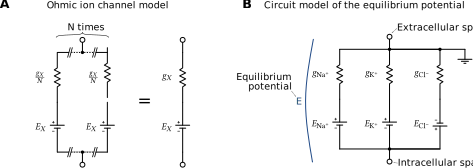
\includegraphics[scale=0.3333]{media/chapters/02_modelling/02_01/electrical_circuit.pdf}
	{\phantomsubcaption\label{fig:electrical_circuit_individual_channels}}
	{\phantomsubcaption\label{fig:electrical_circuit_membrane}}
	\caption[Electrical circuit model of the cell membrane]{Electrical model circuit of the cell membrane.
	\textbf{(A)} Individual ion channels can be modelled as a resistor-voltage-source pair (\emph{left}).
	Instead of modelling all ion channels for the same ion species $X$ independently, they can be mathematically combined into a single pair (\emph{right}).
	\textbf{(B)} Circuit model of a neuron at rest. The ratios of the conductances $g_\mathrm{K^+}$, $g_\mathrm{Na^+}$, and $g_\mathrm{Cl^-}$ determine the cell's equilibrium potential $E$. Arrows indicate the current direction relative to $E = \SI{0}{\volt}$ (not physical ionic flow).}
	\label{fig:electrical_circuit}
\end{figure}
Alternatively, the equilibrium potential can be modelled in terms of the equivalent circuit depicted in \Cref{fig:electrical_circuit}.
The idea is the following.
An ion species $X$ is \enquote{driven} by the voltage difference between the membrane potential \vMem and the reversal potential  $E_X$ (eq.~\ref{eqn:nernst} and \Cref{tbl:nernst}).
Each ion channel provides a conductive path for a specific ion species $X$; however, the channels are tiny, and ionic movement is influenced by thermal Brownian noise.
Hence, there is a chance that ions will collide with the cell interior before passing through a channel.
This provides a resistance $R_X$ to the ionic current \citep{enderle2011bioelectric}.

Each ion channel can thus be modelled electrically as a resistor-voltage-source pair.
The voltage source corresponds to the driving forces that move ions in or out of the cell, whereas the resistor models the stochastic resistance ions encounter while moving through the cell.

Intuitively, the more ion channels that are open---and the larger the permeability $P_X$---the smaller this resistance.
Assuming that $P_X$ represents the number of open channels for an ion species $X$, and that ion channels behave Ohmically, the total ionic current $J_X$ is  (\Cref{fig:electrical_circuit_individual_channels})
\begin{align}
	J_X(v) &= \sum_{i = 1}^{P_X} \frac{\vMem - E_X}{R_X} = \frac{P_X}{R_X} \bigl( \vMem - E_X \bigr) = g_X (\vMem - E_X)\,,
	\label{eqn:ionic_current}
\end{align}
where $g_X$ is the \emph{conductance} of a \enquote{virtual} channel summarizing all $P_X$ channels.%
\footnote{The conductance\index{conductance} $g$ of a resistor (measured in Siemens\index{Siemens}; unit symbol $\si{\siemens} = \si{\per\ohm}$) is the inverse of its resistance $R$.
This unit is commonly used in neuroscience to simplify some equations.
For example, a conductance of zero can be used to describe an open circuit, whereas resistances would take on unwieldy infinite values in this case.}
To obtain the equilibrium potential $E$ for multiple ion channels, we arrange the resistor-voltage-source pairs in parallel (\Cref{fig:electrical_circuit_membrane}).
According to Kirchoff's circuit laws\index{Kirchoff's circuit laws} we have
\begin{align}
	\sum_X J_X(E) = \sum_X g_X (E - E_X) &= 0 \Leftrightarrow E = \frac{\sum_X g_X E_X}{\sum_X g_X} \,, \quad \quad \text{for } \sum_X g_X > 0 \,.
	\label{eqn:circuit_equilibrium}
\end{align}
And for the ion species discussed above we get
\begin{align}
	E &= \frac{g_\mathrm{K^+} E_\mathrm{K^+} + g_\mathrm{Na^+} E_\mathrm{Na^+} + g_\mathrm{Cl^-} E_\mathrm{Cl^-}}{g_\mathrm{K^+} + g_\mathrm{Na^+} + g_\mathrm{Cl^-}} \,,  \quad \quad \text{for } g_\mathrm{K^+} + g_\mathrm{Na^+} + g_\mathrm{Cl^-} > 0 \,.
	\label{eqn:circuit_equilibrium_ions}
\end{align}
Put differently, the equilibrium potential is modelled as a weighted sum of reversal potentials, with the weights being the channel conductances.
However, note that \cref{eqn:ionic_current,eqn:circuit_equilibrium} assume a linear relationship between permeabilities and conductances.
Mathematically, conductance and permeability are two distinct concepts \citep{enderle2011bioelectric}.
Still, although linearity does not follow from the empirically well-tested Goldman equation, the linear approximation preserves the overall qualitative behaviour. We discuss this in more detail in \Cref{app:goldman_equiv_circuit_diff}.

Correspondingly, the above \enquote{equivalent circuit} forms the basis of most neuron models.
The model is simple, conductances can be fit to experimental data, and---as we will see next---the equivalent circuit lends itself to a dynamical description of the cell membrane by simply adding a capacitor to the model circuit.

\pagebreak

\subsection{Neural Dynamics and the Hodgkin-Huxley Model}
\label{sec:neural_dynamics}

We can now describe the steady-state membrane potential of a neuron at rest.
However, the mechanisms discussed so far neither tell us how the membrane potential evolves over time, nor do they describe the action potential---the phenomenon distinguishing most neurons from other cells in the first place.

Fundamentally, neural dynamics can be summarised as follows.
Assume that we inject short positive current pulses $J(t)$ into a neuron using a microelectrode.
Measuring the membrane potential $\vMem(t)$ over time $t$ we observe the following:
\begin{enumerate}[1.]
	\setlength{\itemsep}{0.25em}
	\vspace*{-0.25em}
	\item \emph{Subthreshold dynamics.} Small current pulses charge the cell membrane over time. The membrane potential \vMem rises while the input persists, and then decays back to \vRest (\Cref{fig:action_potentials_subthreshold}).
	\item \emph{Superthreshold dynamics.} If the current pulse is energetic enough for the membrane potential to reach a soft threshold value $v_\mathrm{th}$, the neuron generates an action potential; \vMem suddenly rises towards positive numbers (\emph{depolarisation}\index{neuron!depolarisation}), and then falls to voltages below \vRest (\emph{repolarisation}\index{neuron!repolarisation})---the neuron is \emph{hyperpolarised}\index{neuron!hyperpolarisation}. Over time, \vMem converges back to  \vRest.  This is depcited in \Cref{fig:action_potentials_superthreshold}.
	\item \emph{Refractory period.} While the neuron is hyperpolarised, it is significantly harder to evoke another action potential. This phase is referred to as the \emph{refractory period}\index{neuron!refractory period} (\Cref{fig:action_potentials_refractory}).%
	\footnote{Technically, modellers distinguish between \emph{absolute} and \emph{relative} refractory periods. During the absolute refractory period the neuron cannot produce action potentials; during the relative refractory period merely large input currents are required \citep[Section~2.3.2]{izhikevich2007dynamical}.}
\end{enumerate}

\vspace*{-0.25em}
The first model to provide a detailed mechanistic account of these observations---and indeed what we used as a stand-in for a real neuron in the above exploration---is the Hodgkin-Huxley model \citep{hodgkin1952quantitative}.
This model has been exceptionally successful in predicting neural behaviour quite accurately, and forms a basis for a whole family of neuron models \citep{meunier2002playing,mccormick2007hodgkin}.

The important idea of Hodgkin-Huxley-type models is that the channel conductances $g_\mathrm{K^+}$ and $g_\mathrm{Na^+}$ possess dynamics that nonlinearly depend on the current membrane potential.%
\footnote{Hodgkin-Huxley-type models are sometimes also called \enquote{conductance-based neurons}. This is not to be confused with \enquote{conductance-based synapses}---synapse models are independent of the neuron model.}
That is, the permeability of the membrane for potassium and sodium changes depending on the membrane potential due to voltage-dependent ion channels.
Hodgkin and Huxley model the dynamics of these channels using three dimensionless \enquote{gating} variables $m(t)$, $h(t)$, $n(t)$.
Revised models differ from the original in terms of the concrete dynamics of these variables.
In our examples, we use dynamics adapted from a model of pyramidal cells in the hippocampus described by \citet[Chapter~4, pp.~92-94; \Cref{app:hippocampal_hh}]{traub1991neuronal}.

\begin{figure}[p]
	\includegraphics{media/chapters/02_modelling/02_01/action_potentials.pdf}
	{\phantomsubcaption\label{fig:action_potentials_subthreshold}}
	{\phantomsubcaption\label{fig:action_potentials_superthreshold}}
	{\phantomsubcaption\label{fig:action_potentials_refractory}}
	\caption[Hodgkin-Huxley-type model neuron simulations demonstrating action potential generation]{Hodgkin-Huxley-type model neuron simulations demonstrating action potential generation (using the dynamics described by \cite{traub1991neuronal}).
	% This figure was in part inspired by \citet[Figure~2.15, p.~45]{izhikevich2007dynamical}
	\textbf{(A)} Injecting a current $J$ into the neuron (orange; \emph{bottom}) charges the cell membrane. As long as the membrane potential $v$ (\emph{top}) approximately stays below a threshold, the neuron does not generate action potentials; the membrane acts linearly. \textbf{(B)} Above a certain threshold, the neuron suddenly generates an action potential. \textbf{(C)} Directly after an action potential, during the \emph{refractory period}, even large input currents cannot evoke action potentials.}
\end{figure}

\begin{figure}[p]
	\vspace{0.5cm}
	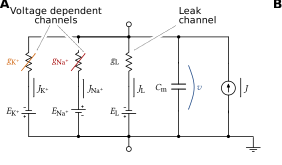
\includegraphics[scale=0.3333]{media/chapters/02_modelling/02_01/hodgkin_huxley_circuit.pdf}~~~~%
	\includegraphics{media/chapters/02_modelling/02_01/action_potentials_hh_conductances.pdf}
	{\phantomsubcaption\label{fig:action_potentials_hh_conductances_circuit}}
	{\phantomsubcaption\label{fig:action_potentials_hh_conductances_conductances}}
	\vspace{-0.5cm}
	\caption[Equivalent circuit diagram of the Hodgkin-Huxley model]{Equivalent circuit diagram of the Hodgkin-Huxley model. \textbf{(A)} Equivalent circuit model of the Hodgkin-Huxley model. The resting potential is generated by a virtual \enquote{leak} channel; the $\mathrm{K}^+$ and $\mathrm{Na}^+$ channels vary over time and depend on the membrane potential. \textbf{(B)} Conductance traces for a single action potential (slice from \cref{fig:action_potentials_superthreshold}). Sodium drives depolarisation, potassium repolarisation.}
	\label{fig:action_potentials_hh_conductances}
\end{figure}

Conveniently, Hodgkin-Huxley-type models are an extension of the equivalent cell-membrane circuit from the previous subsection (\Cref{fig:electrical_circuit}).
We just need to make two conceptual changes to account for the linear subthreshold and nonlinear superthreshold dynamics.

\subsubsection{Subthreshold dynamics}
To model the linear subthreshold dynamics, we simply add a capacitor with capacitance $C_\mathrm{m}$ to the circuit model.
This \emph{membrane capacitance}\index{neuron!membrane capacitance} is physically motivated by the cell membrane separating two electrically charged bodies.
Any such system inherently possesses capacitive properties.%
\footnote{To be clear, the membrane capacitance is not specific to the Hodgkin-Huxley model. In fact, this assumption preceded the Hodgkin-Huxley model by several decades (e.g., \cite{lapicque1907recherches}). We discuss the corresponding LIF neuron model first proposed by Lapicque later in this chapter.}
Given an input current $J(t)$, the sub-threshold dynamics can be described in terms of the following differential equation
\begin{align}
	\begin{aligned}
	\CMem \dot\vMem(t) &=
		  g_\mathrm{K^+} \bigl(E_\mathrm{K^+} - \vMem(t)\bigr)
		+ g_\mathrm{Na^+} \bigl(E_\mathrm{Na^+} - \vMem(t)\bigr)
		+ g_\mathrm{Cl^-} \bigl(E_\mathrm{Cl^-} - \vMem(t)\bigr) + J(t) \\ &=
	g_\mathrm{L} \bigl(\EL - \vMem(t)\bigr) + J(t) \,.
	\end{aligned}
\end{align}
The last term simplifies the dynamics using a \emph{leak conductance} \gL and \emph{leak potential} \EL that form a basic resistor-capacitance (RC) circuit (right half of \Cref{fig:action_potentials_hh_conductances_circuit}) with the time-constant $\tauMem = \CMem g_\mathrm{L}^{-1}$.
We have
\begin{align*}
	\gL &= g_\mathrm{K^+} + g_\mathrm{Na^+} + g_\mathrm{Cl^-} \,, &
	\text{and} \quad \quad \EL &= \frac{g_\mathrm{K^+} E_\mathrm{K^+} +
				 	g_\mathrm{Na^+} E_\mathrm{Na^+} + g_\mathrm{Cl^-} E_\mathrm{Cl^-}}{g_\mathrm{K^+} + g_\mathrm{Na^+} + g_\mathrm{Cl^-}} \,.
\end{align*}
The equation for \EL is exactly the equilibrium potential as per \cref{eqn:circuit_equilibrium_ions}.
In the absence of an input current $J(t)$, \EL is a stable attractor in the subtreshold dynamics.
It typically holds $\vRest = \EL$; still, we use \EL in this context to emphasise its use as a conductance-based channel.

\subsubsection{Superthreshold dynamics}
The superthreshold dynamics are responsible for action potential generation.
We describe these nonlinear dynamics in terms of potassium and sodium channels with time-dependent conductances $g_\mathrm{K^+}(t)$, $g_\mathrm{Na^+}(t)$ (\Cref{fig:action_potentials_hh_conductances_circuit}):
\begin{align*}
	\CMem \dot\vMem(t) &=
		  g_\mathrm{K^+}(t) \bigl(E_\mathrm{K^+} - \vMem(t)\bigr)
		+ g_\mathrm{Na^+}(t) \bigl(E_\mathrm{Na^+} - \vMem(t)\bigr)
		+ g_\mathrm{L} \bigl(\EL - \vMem(t)\bigr) + J(t) \,.
\end{align*}
Hodgkin and Huxley define the time-course of these conductances in terms of a dynamical system of gating variables $m(t)$, $h(t)$, and $n(t) \in [0, 1]$ that in turn depend on $\vMem(t)$.
We have
\begin{align*}
	g_\mathrm{K^+}(t) &= \hat g_\mathrm{K^+} n(t)^4 \,, &
	g_\mathrm{Na^+}(t) &= \hat g_\mathrm{Na^+} m(t)^3 h(t) \,,
\end{align*}
where $\hat g_\mathrm{K^+}$ and $\hat g_\mathrm{Na^+}$ are the maximum conductances.
%Using place-holder functions $f_m$, $f_n$, $f_h$, the dynamics of the gating variables are
%\begin{align*}
%	\dot m(t) &= f_m(v(t), m(t)) \,, &
%	\dot h(t) &= f_h(v(t), h(t)) \,, &
%	\dot n(t) &= f_n(v(t), n(t)) \,.
%\end{align*}
The dynamics of the gating variables (cf.~\Cref{app:hippocampal_hh}) produce a tight feedback loop between $\vMem(t)$ and the conductances.

\Cref{fig:action_potentials_hh_conductances_conductances} depicts the resulting conductances over time.
In particular, $g_\mathrm{Na^+}(t)$ rises rapidly once a certain threshold potential is exceeded.
This drives the cell towards the positive sodium reversal potential $E_\mathrm{Na^+}$; the cell becomes depolarised.
In turn, the positive membrane potential triggers a rise in potassium conductivity $g_\mathrm{K^+}(t)$, while the gating variable $h(t)$ shuts the sodium current off. This drives the cell towards the negative potassium reversal potential $E_\mathrm{K^+}$; the cell becomes hyperpolarised, while the potassium conductance remains relatively high for a short time.
This accounts for refractoriness, as large $J$ are required to counter the potassium current.

A detailed description of the superthreshold dynamics is provided in \Cref{app:hippocampal_hh}, including the unabridged equations and additional diagrams.
An even more thorough discussion of the dynamics of Hodgkin-Huxley-like neurons may be found in \citet{izhikevich2007dynamical}.

\subsection{Compartmental Neuron Models}

\begin{figure}
	\centering
	\includegraphics{media/chapters/02_modelling/02_01/compartments.pdf}
	{\phantomsubcaption\label{fig:compartments_physical}}%
	{\phantomsubcaption\label{fig:compartments_volumes}}%
	{\phantomsubcaption\label{fig:compartments_circuit}}%
	\caption[Equivalent circuit of an exemplary compartmental neuron model]{Equivalent circuit diagram of an exemplary compartmental neuron model. \textbf{(A)} A biological neuron is divided into $N = 6$ individual compartments (neuron redrawn from \cite{howell1916textbook}, Figure~84, p.~187).
	\textbf{(B)} Compartments are often approximated as cylinders; using \enquote{cable theory} one can compute how potentials propagate along the membrane.
	\textbf{(C)} Cylinder models can be further simplified by modelling each compartment as a simple equivalent circuit. Here, the somatic compartment (orange) possesses Hodgkin-Huxley-like voltage-dependent dynamics. Individual model circuits are resistively coupled with conductances $g_{ij}$.
	}
	\label{fig:compartments}
\end{figure}

As we saw at the beginning of this section, neurons possess intricate morphologies (cf.~\Cref{fig:compartments_physical}).
Up to this point, we have minimised this fact and instead summarised neural electrophysiology in terms of a single membrane potential over time, $\vMem(t)$.
Models based on this assumption are referred to as \emph{point neurons} or \emph{single compartment models}.

The spatial organization of a neuron can have a significant impact on its function.
This is because the intracellular fluid is not a particularly good electrical
conductor.
Hence, in combination with the capacitive properties of the membrane, we can, at a single point in time, measure different membrane potentials throughout the neuron.
These voltage differences cause currents injected at different points of the neuron to interact nonlinearly, which supports computation.
Perhaps confusingly, the neural \emph{dynamics} we describe here are mostly linear, but the \emph{average effect over time} is nonlinear.
We discuss this in more detail in the next chapter.

\begin{figure}
	\includegraphics{media/chapters/02_modelling/02_01/cylinder.pdf}
	\caption[Illustration of potential propagation within a cylindrical cable.]{Illustration of potential propagation within a cylindrical cable. Injecting a \SI{1}{\nano\ampere} current at the centre of a \SI{1}{\milli\metre} long cable (diameter \SI{1}{\micro\metre}, capacitance \SI{1}{\micro\farad\per\square\centi\metre}, longitudinal resistance \SI{150}{\ohm\per\centi\metre}, leak conductance \SI{0.5}{\milli\siemens\per\square\centi\metre}). \textbf{(A)} Potential at different points $x$ and times $t$ (see \emph{(B)} for a legend) in a linear cable. \textbf{(B)} Continuous representation of the same data; see \emph{(A)} for the mapping between colours and voltages.}
	\label{fig:cylinder}
\end{figure}

A quite faithful model of this can be constructed using \emph{cable theory}.
To this end, individual neurons are approximated as an arrangement of cylinders that represent individual segments of the neuron (\Cref{fig:compartments_volumes}).
Voltages spatially propagate through these cylinders. That is, the model takes the longitudinal resistance of the individual neuron segments as well as their capacitative properties into account.
Given an input impulse, we can use \emph{cable equations} to predict the voltage $v(x, t)$ at a certain position $x$ along the segment at a time $t$ (cf.~\Cref{fig:cylinder}).
Mathematically, this can be accomplished by assuming an infinite number of resistively coupled RC circuits and solving a partial differential equation \citep[Chapter~2]{koch1999biophysics}.


Instead of modelling spatial propagation of voltages through cylinders, individual cylinders can be approximated as one or multiple instances of the underlying equivalent circuit.
Each of these instances is referred to as a \emph{compartment} (\Cref{fig:compartments_circuit}).
Such neuron models are correspondingly called \emph{multi-compartment} or \emph{compartmental} neuron models.
In theory, the number of compartments $N$ determines how closely the model can be made to match empirical data---some detailed neuron models rely on thousands of individual segments.
However, for most network-level research, compartments can often be joined into reduced models that capture most of the original neural behaviour \citep{herz2006modeling}.

Depending on the modelling assumptions, compartments may either be \emph{active} or \emph{passive}.
Active compartments---such as the \enquote{somatic} compartment in \Cref{fig:compartments_circuit}---model superthreshold dynamics and are capable of producing spikes, for example by including voltage-dependent Hodgkin-Huxley type models.
In contrast, passive compartments are typically modelled as the simple linear subthreshold RC-circuit.
A more detailed description of such models, including the passive dendritic trees we discuss later, is given by \citet[Chapter~3]{koch1999biophysics}.

If we assume that individual neural compartments are resistively coupled, the current $J_i(t)$ flowing into the $i$th compartment is, according to Kirchhoff's circuit laws, given as
\begin{align}
	J_i(t) &= \sum_{j = 1}^N c_{ij} \bigl(v_j(t) - v_i(t)\bigr) \,.
	\label{eqn:multi_comp_current}
\end{align}
Here, $c_{ij} = c_{ji}$ is the conductance between the $i$th and $j$th compartment. A value of $c_{ij} = 0$ indicates no connection.
Mathematically, the conductances $c_{ij}$ correspond to the symmetric adjacency matrix of an undirected connectivity graph describing the compartmental model.


\clearpage
\setcounter{section}{1}
% !TeX spellcheck = en_GB

\section{From Individual Neurons to Spiking Neural Networks}
\label{sec:neuron_models}

The equations from the previous section model the basic electrophysiological properties of individual neurons.
Of course, a single neuron on its own does not give rise to animal behaviour.
Hence, in this section, we discuss how individual neurons can be used to form neural networks.
We provide an overview of synaptic transmission, the process underpinning neural information transfer, followed by a discussion of idealised neuron and synapse models that lessen the computational burden of simulating biological systems.
We close with a short discussion of spiking neural networks and population tuning---the latter shedding some light onto the role that individual neurons play in a network.


\subsection{Synaptic Transmission}
\label{sec:synaptic_transmission}

So far, our descriptions of neural dynamics assumed that neurons receive inputs through artificially injected currents $J(t)$.
%While this can be experimentally achieved using a microelectrode and a precision power supply,
Of course, this does not explain how neurons receive inputs \emph{in vivo}.
As we mentioned in our overview in \Cref{sec:neurons_overview}, the interface between two neurons is called a \emph{synapse}.
Neuroscientists distinguish two synapse types: electrical and chemical.


\subsubsection{Electrical synapses}
In adult vertebrates, electrical synapses are much less common than chemical synapses.
Still, they play an important role in some mammalian brain areas, including the retina and the inferior olive in the cerebellum \citep[Chapter~5]{meriney2019synaptic}.

Electrical synapses directly connect two neurons through specialised ion channels, so-called \emph{gap junctions}.
These channels typically allow a bidirectional exchange of ions between the intracellular fluids.
Correspondingly, neurons connected via gap junctions can be modelled using the same techniques as multi-compartment models (eq.~\ref{eqn:multi_comp_current}; \cite{kandel2012principles}, Chapter~8).

\subsubsection{Chemical synapses}
Neurons coupled via chemical synapses are electrically isolated.
The synapse establishes a unidirectional information flow and only passes on superthreshold signals.
The transmitting and receiving neurons are generally referred to as \enquote{pre-synaptic} and \enquote{post-synaptic neurons}, respectively.
To save some space, we use the terms pre- and post-neurons.
Similarly, the synapse is divided into the \enquote{pre-} and \enquote{post-synapse}.

\begin{figure}
	\includegraphics{media/chapters/02_modelling/02_02/synapse.pdf}%
	\caption[Synaptic transmission in a chemical synapse]{Synaptic transmission in a chemical synapse. Grey line in the membrane potential traces is the spike onset. See text for a description. Inspired by \citet[Figure~8-8B-C, p.~185]{kandel2012principles}.}
	\label{fig:synapse}
\end{figure}

As illustrated in \Cref{fig:synapse}, action potentials arriving at axon terminal, trigger the release of \emph{neurotransmitter} molecules.
These traverse the nanometer-scale gap between the pre- and post-synapse, the \emph{synaptic cleft}, and temporarily bind to post-synaptic receptors specific to that neurotransmitter type.
This---directly or indirectly---causes ion channels in the post-neuron to open.
In turn, the permeability of the post-neuron for that particular ion species changes.

¸The resulting synaptically mediated membrane potential fluctuations are called \emph{post-synaptic potentials} (\PSPpl).
Depending on the type of ion channels opened or closed, the \PSP can either drive the neuron towards more positive voltages (if sodium channels are opened), or negative voltages (e.g., if potassium or chloride channels are opend).
Positive \PSPpl are referred to as \emph{excitatory} (\EPSP), negative changes as \emph{inhibitory} (\IPSP).
%Correspondingly, we distinguish excitatory and inhibitory post-synaptic potentials (EPSPs) and (IPSPs).

Whether a pre-neuron acts excitatorily or inhibitorily on a post-neuron depends on the kind of neurotransmitter released by the pre-neuron, as well as the specific receptors and ion channels in post-neuron.
%Typically, each neurotransmitter either has an inhibitory or excitatory effect.
For example, the Gamma-Aminobutyric acid (GABA) neurotransmitter is primarily inhibitory (via GABA\textsubscript{A} or GABA\textsubscript{B} receptors), whereas Glutamic acid (Glutamate) is mostly excitatory (via AMPA or NMDA receptors; \cite{kandel2012principles}, Chapter~10).

Importantly, the mixture of neurotransmitters is the same across all axonal branches of a neuron.
This is known as \emph{Dale's principle} \citep{strata1999dale,eccles1986chemical}.
Put simply, individual neurons typically either act excitatorily or inhibitorily on their post-neurons.%
\footnote{This characterisation of Dale's principle is useful, but technically incorrect. For example, a pre-synapse releasing glutamate typically excites post-neurons, but inhibits special neurons with inhibitory glutamate receptors \citep{cleland1996inhibitory}.
Additionally, synapses could release both excitatory and inhibitory neurotransmitters.
}
We hence refer to neurons---and not just individual synapses---as being excitatory or inhibitory.

\begin{figure}
	\centering
	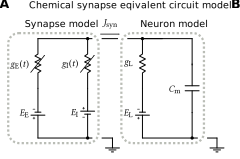
\includegraphics[scale=0.3333]{media/chapters/02_modelling/02_02/synapse_model.pdf}%
	\includegraphics{media/chapters/02_modelling/02_02/synapse_model_traces.pdf}%
	{\phantomsubcaption\label{fig:synapse_model_circuit}}%
	{\phantomsubcaption\label{fig:synapse_model_traces}}%
	\caption[The conductance-based synapse model]{The conductance-based synapse model.
	\textbf{(A)} Circuit diagram of a passive cell membrane with synaptically controlled excitatory and inhibitory conductance-based channels.
	\textbf{(B)} Illustrative voltage, current, and conductance traces. \emph{Top:} Excitatory and inhibitory channel conductances after a pre-synaptic action potential (grey dashed line). \emph{Middle:} Resulting excitatory and inhibitory post-synaptic potentials. \emph{Bottom:} Corresponding excitatory and inhibitory post-synaptic currents.}
	\label{fig:synapse_model}
\end{figure}

\subsubsection{Conductance-based chemical synapse model}
Most gated ion channels can be modelled as a voltage-resistor pair with variable conductance per receptor type \citep{roth2009modeling}.
This is depicted in \Cref{fig:synapse_model} for generic \enquote{excitatory} and \enquote{inhibitory} receptors.
Mathematically, the post-synaptic current $J_\mathrm{syn}(t)$ flowing from the synapse into the neuron is given as
\begin{align}
	J_\mathrm{syn}(t) &=
		  g_\mathrm{E}(t) \bigl(E_\mathrm{E} - v(t)\bigr)
		+ g_\mathrm{I}(t) \bigl(E_\mathrm{I} - v(t)\bigr) \,.
	\label{eqn:conductance_synapse}
\end{align}
Here, $E_\mathrm{E}$ and $E_\mathrm{I}$ are the equilibrium potentials of the gated ion channels.
These potentials are not necessarily equal to ion reversal potentials (\Cref{tbl:nernst}).
For example, NMDA and AMPA channels conduct both $\mathrm{Na^+}$ and $\mathrm{K^+}$, resulting in $E_\mathrm{E} \approx \SI{0}{\milli\volt}$ \citep[Chapter~10]{kandel2012principles}.
%All receptors with the same reversal potential are summarised as single channel in the equivalent circuit.
%Correspondingly, $g_\mathrm{E}$ and $g_\mathrm{I}$ are the sum over the state of multiple post-neurons (similar to \Cref{fig:electrical_circuit_individual_channels}).

\subsubsection{Synaptic dynamics and weights}
The time course of the conductance $g(t)$ depends on the neurotransmitter and receptor type.
Generally speaking, as illustrated in \Cref{fig:synapse_model_traces}, the conductance rises quickly after a spike is received, and decays slowly as the neurotransmitter unbinds from the receptors.
Receptors directly controlled by neurotransmitters acting as ligands (\Cref{fig:synapse}) tend to have relatively short time-constants between $1$ and \SI{100}{\milli\second} \citep{jones2014neurotransmitter}.
Some receptors (e.g., \enquote{metabotropic receptors}) rely on indirect chemical cascades, leading to longer time-constants \citep[Chapter~14]{meriney2019synaptic}; this is not captured well by the models we present here \citep{roth2009modeling}.

\begin{figure}
	\includegraphics{media/chapters/02_modelling/02_02/synapse_filter_examples.pdf}
	{\phantomsubcaption\label{fig:synapse_filter_examples_time_constants}}%
	{\phantomsubcaption\label{fig:synapse_filter_examples_traces}}%
	\caption[Second- and first-order exponential synaptic low-pass filter dynamics]{Illustration of the second- and first-order exponential synaptic low-pass filter dynamics. \textbf{(A)} Impulse response of the second-order dynamics for different $\tau_1$ and $\tau_2$. \emph{Top:} visualisation of the time-constants used below. Swapping $\tau_1$ and $\tau_2$ does not change the dynamics (grey crosses). \emph{Bottom:} Impulse response of the filters (responses normalised to equal area), circles are the peaks. \textbf{(B)} Illustration of post-synaptic conductance traces (\emph{bottom}) according to \Cref{eqn:low_pass_second_order,eqn:low_pass_first_order} for two pre-neurons producing action-potentials (\emph{top}) connected with two different synaptic weights $w_1$, $w_2$.}
\end{figure}

Ligand-gated receptor dynamics are often modelled as a second-order linear dynamical system.
Let $t_{ij}$ denote the time of the $j$th pre-synaptic spike arriving from the $i$th pre-neuron, and let $\tau_1$, $\tau_2$ denote the rise and delay times (\Cref{fig:synapse_filter_examples_time_constants}).
We have \citep{roth2009modeling}:
\begin{align}
	\dot g_1(t) &= -\frac{g_1(t)}{\tau_\mathrm{1}} + g_2(t) \,, &
	\dot g_2(t) &= -\frac{g_2(t)}{\tau_\mathrm{2}} + \sum\nolimits_{i} \alpha w_i \sum\nolimits_{j} \delta(t_{ij} - t) \,,
	\label{eqn:low_pass_second_order}
\end{align}
where $\delta(t)$ is the Dirac-delta, and $\alpha$ is a scaling factor such that the scalar $w_i$ corresponds to the peak value of $g_1(t)$ for a single action potential received from pre-neuron $i$ (\Cref{fig:synapse_filter_examples_traces}).
For $\tau_1 = \tau_2$ this type of synaptic dynamics follow the so-called \emph{alpha function}.

Notably, the scalar $w_i$ is referred to as \emph{synaptic weight} in computational modelling, or as \emph{synaptic strength} in neuroscience.
This scalar summarises various biological processes that determine the average response of the post-neuron to an action-potential received from the $i$th pre-neuron.
For example, synaptic strength can depend on the amount of neurotransmitter released in the pre-synapse, or the ion-channel density in the post-synapse \citep[Chapter~12]{kandel2012principles}.
In this context, the term \emph{synaptic plasticity} refers to a change in synaptic strength over time.
This plays a key role in learning---we discuss this in more detail in Chapter~5.


Typically, the rise-time of $g(t)$ is relatively short.
Correspondingly, the second-order low-pass filter can be approximated by a first-order dynamical system with decay-time $\tau$.
Mathematically, and as depicted the lower portion of \Cref{fig:synapse_filter_examples_traces}, the dynamics are
\begin{align}
	\dot g(t) &= -\frac{g(t)}{\tau} + \sum\nolimits_{i}  w_i \sum\nolimits_{j} \delta(t_{ij} - t) \,.
	\label{eqn:low_pass_first_order}
\end{align}

\subsubsection{Synaptic dynamics as filters}
The above synaptic dynamics (eqs.~\ref{eqn:low_pass_second_order}, \ref{eqn:low_pass_first_order}) are linear time-invariant (\LTI) systems.
%of the form $\dot{\vec g}(t) = \mat A{\vec g(t)} + \mat B u(t)$, where $\mat A \in \mathbb{R}^{n \times n}$ is a state-transition matrix, $\mat B \in \mathbb{R}^{n \times 1}$ is the input matrix, and $u(t)$ is the input in the form of weighted pre-synaptic spike events; the output of the system (i.e., the conductance) is simply the first state-dimension $g_1$.
\LTI systems are fully characterised by their \emph{impulse response} $h(t)$ and can be replaced by a convolution (\enquote{$\ast$}) between $h(t)$ and the weighted input spike-train $u(t)$:
\begin{align}
	g(t)
		&= (h \ast u)(t)
		 = \int_0^\infty h(\tau) u(t - \tau) \,\mathrm{d}\tau
		 = \int_0^\infty h(\tau) \sum\nolimits_{i}  w_i \sum\nolimits_{j} \delta(t_{ij} - \tau) \,\mathrm{d}\tau \,.
	\label{eqn:synapse_impulse}
\end{align}
For the first-order dynamics in \cref{eqn:low_pass_first_order}, the impulse response is $h(t) = \exp(-t/\tau)$ for $t \geq 0$ (and $h(t)= 0$ if $t < 0$); impulse responses of the second-order system are depicted in \Cref{fig:synapse_filter_examples_time_constants}.
Convolutions such as \cref{eqn:synapse_impulse} can alternatively be expressed as multiplication of the frequency contents of the impulse response $h(t)$ and the input spike-train $u(t)$:
\begin{align}
	g(t) &= \mathcal{F}^{-1} \bigl(\mathcal{F}(h) \mathcal{F}(u) \bigr)(t) \,,
\end{align}
where $\mathcal{F}$ is the forward Fourier transformation, and $\mathcal{F}^{-1}$ its inverse.
From this signal-processing perspective, the synaptic dynamics attenuate frequencies in the input spike-train; they act as a \emph{filter}.
The synaptic dynamics discussed so far attenuate low frequencies far less than higher frequencies; they are thus referred to as \emph{low-pass filters}.

% TODO: Talk about filters in general
% TODO: Provide some example synaptic time constants

\newpage

\subsection{Simplified Neuron Models}
\label{sec:simplified_neuron_models}

The models discussed in the previous section describe indiviudal neurons at a relatively low level of abstraction.
This incurs a high computational cost, especially when considering detailed compartemental neurons with Hodgkin-Huxley-like super-threshold dynamics.

Fortunately, important electrophysiological properties of neurons can be captured by less detailed, computationally inexpensive, models \citep[cf.][Chapter~14]{koch1999biophysics}.
For example, the Izhikevich \citep{izhikevich2004which} and Adaptive Exponential \citep{brette2005adaptive} point neuron models require only two state variables, but are capable of reproducing spike patterns observed in nature.
Here, we focus on the even simpler \enquote{leaky integrate-and-fire} (\LIF) model.

\subsubsection{The leaky integrate-and-fire model}

\begin{figure}[t]
	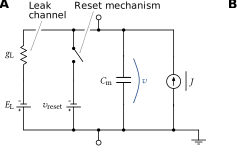
\includegraphics[scale=0.3333]{media/chapters/02_modelling/02_02/lif_circuit.pdf}%
	\kern-0.25cm\includegraphics{media/chapters/02_modelling/02_02/lif_traces.pdf}
	\caption[Equivalent circuit diagram and membrane potential trace of a LIF neuron]{Equivalent circuit diagram and membrane potential trace of a \LIF neuron. \textbf{(A)} The \LIF model consists of a capacitative membrane with a \enquote{leak} channel. A reset mechanism clamps \vMem to the reset potential \vReset. \textbf{(B)} Membrane potential trace (\emph{top}) for rectangle pulse current inputs (\emph{middle}).  Vertical dashed lines are spike events. The bottom graph depicts the remaining refractory period.}
	\label{fig:lif}
\end{figure}

%\footnote{Extensions to the LIF model include the quadratic and exponential integrate-and-fire models (QIF and EIF, respectively). Hence, LIF is sometimes read as \enquote{linear integrate-and-fire}. Furthermore, there is the IF model, that does not include a leak channel, sometimes also called nLIF (non-leaking).}
A variant of the \LIF model---lacking refractoriness---dates back to \citet{lapicque1907recherches}.
Just like the Hodgkin-Huxley model (\Cref{sec:neural_dynamics}), the \LIF neuron is based on a capacitive membrane with a leak channel.
The input current is integrated by the capacitor, which, at the same time, is discharged through the leak channel:
\begin{align}
	\CMem \dot{\vMem}(t) =
		\gL \bigl(\EL - \vMem(t)\bigr) + J(t) \,,
	\label{eqn:lif}
\end{align}
where \gL is the leak conductance, \EL is the leak reversal potential, and $J(t)$ is a (synaptic) current injected into the membrane.
Unlike the Hodgkin-Huxley model, the dynamics of the system do not model spike production; \enquote{firing} is handled outside the dynamical system. 
Once $\vMem(t)$ reaches a threshold $\vTh$, a spike event is recorded and \vMem is held at the \emph{reset potential} \vReset for the duration of the refractory period \tauRef.
This is depicted in \Cref{fig:lif}.

\subsubsection{Response curve}

\begin{figure}
	\centering
	\includegraphics{media/chapters/02_modelling/02_02/neuron_voltage_traces.pdf}
	\caption[Voltage traces for the LIF and Hodgkin-Huxley neuron model]{Voltage traces (\emph{top}) for the \LIF and a Hodgkin-Huxley-type neuron dynamics described by \citet{traub1991neuronal} given a current ramp input~(\emph{bottom}). Dashed vertical lines correspond to spike events. Dotted line is the resting potential at $\EL=\SI{-65}{\milli\volt}$. Both neurons have a membrane capacitance of $C_\mathrm{m} = \SI{200}{\pico\farad}$ and a leak conductance of $g_\mathrm{L} = \SI{10}{\nano\siemens}$. \textbf{(A)} The \LIF neuron model does not account for spike production; the voltage is simply reset to $v_\mathrm{reset} = \SI{-85}{\milli\volt}$ for $\tauRef = \SI{2}{\milli\second}$ once the membrane potential passes the threshold at $v_\mathrm{th} = -\SI{55}{\milli\volt}$. \textbf{(B)} Same experiment for a Hodgkin-Huxley neuron. Notably, the super-threshold dynamics of the Hodgkin-Huxley model action potentials and the first spike appears significantly earlier compared to the \LIF neuron.}
	\label{fig:neuron_voltage_traces}
\end{figure}

\begin{figure}
	\centering
	\includegraphics{media/chapters/02_modelling/02_02/neuron_response_curves.pdf}%
	{\phantomsubcaption\label{fig:neuron_response_curves_lif}}%
	{\phantomsubcaption\label{fig:neuron_response_curves_hh}}%
	\caption[Response curves for the LIF and Hodgkin-Huxley-type neuron model]{Response curves (also called IF-curves) $G[J]$ for the \LIF and Hodgkin-Huxley-type neuron model from \Cref{fig:neuron_voltage_traces}. Data extracted from the inter-spike-intervals of a current ramp experiment (sweep from \SIrange{0}{2}{\nano\ampere} over ten seconds at a \SI{10}{\micro\second} resolution). Although the \LIF and Hodgkin-Huxley models have drastically different dynamics, their response curves are qualitatively similar.}
	\label{fig:neuron_response_curves}
\end{figure}

\begin{figure}
	\centering
	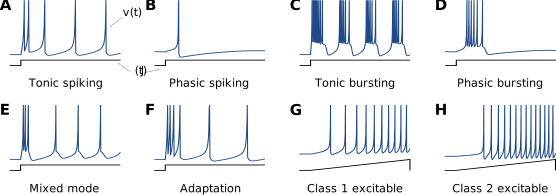
\includegraphics{media/chapters/02_modelling/02_02/izhikevich_whichmod_figure1.pdf}%
	{\phantomsubcaption\label{fig:izhikevich_whichmod_figure1a}}%
	{\phantomsubcaption\label{fig:izhikevich_whichmod_figure1b}}%
	{\phantomsubcaption\label{fig:izhikevich_whichmod_figure1c}}%
	{\phantomsubcaption\label{fig:izhikevich_whichmod_figure1d}}%
	{\phantomsubcaption\label{fig:izhikevich_whichmod_figure1e}}%
	{\phantomsubcaption\label{fig:izhikevich_whichmod_figure1f}}%
	{\phantomsubcaption\label{fig:izhikevich_whichmod_figure1g}}%
	{\phantomsubcaption\label{fig:izhikevich_whichmod_figure1h}}%
	\caption[Diversity of neural dynamics for constant or ramp input currents]{Diversity of neural dynamics for constant or ramp input currents. Each plot depicts membrane-potential traces $v(t)$ (\emph{top}) of the Izhikevich neuron model (with different parameters) for an input current $J(t)$ (\emph{bottom}). \LIF neurons are only capable of behaviours \emph{A} and \emph{G}. Partially reproduced (dynamics for input pulses were skipped) with minor modifications from \citet{izhikevich2004which}. Electronic version of the figure and reproduction permissions freely available at \url{http://www.izhikevich.org}.}
	\label{fig:izhikevich_whichmod_figure1}
\end{figure}

\Cref{fig:neuron_voltage_traces} depicts a comparison between the Hodgkin-Huxley-type and \LIF dynamics.
The reset and threshold potential of the \LIF neuron model have been tuned to match the sub-threshold membrane potentials observed in the Hodgkin-Huxley neuron.
In both cases---apart from the obviously missing super-threshold dynamics---the inter-spike-interval decreases the larger $J$, leading to a higher spike rate.
This suggests a characterisation of neurons in terms of their \emph{response curve} $G[J]$ (\Cref{fig:neuron_response_curves})
\begin{align}
	G[J] &= \lim_{T \to \infty} \frac{n_\mathrm{spikes}(J, T)}{T} \,, & \text{where } n_\mathrm{spikes}(J, T) &= \text{\#spikes for input $J$ over a period $T$} \,.
	\label{eqn:response_curve}
\end{align}
Of course, this only makes sense if we assume that the neuron has a non-zero steady-state activity for a constant superthreshold input current.
This is not necessarily true; neurons can exhibit complex behaviours that violate this assumption \citep{izhikevich2004which}.
For example, \emph{phasic} neurons only produce a limited number of spikes in response to an input step (Figure~\ref{fig:izhikevich_whichmod_figure1}B, D, E), while other neurons adapt to constant input currents over time, resulting in a reduction in frequency (Figure~\ref{fig:izhikevich_whichmod_figure1}F).
Still, neurons often behave \emph{tonically} (Figure~\ref{fig:izhikevich_whichmod_figure1}A, C, G, H), and can be reasonably well characterised in terms of a response curve.

Response curves and time-less \enquote{rate neurons} form the basis for artificial neural networks commonly used in machine learning. We discuss this in more detail later in this thesis.
Furthermore, we revisit temporal properties of the response curve when we discuss temporal tuning curves. % LEAVE SPACE HERE
% TODO add section references

\subsubsection{LIF response curve}
For most neuron models, it is impossible to derive a closed-form expression for the average spike rate $G[J]$ given a constant current $J$; there typically is no closed-form solution for $G[J]$. 
%\footnote{Very few differential equations posses closed-form solutions. Even slightly more complex models (e.g.,~first-order current-based synapses instead of constant $J$) require the analytic Lambert $\mathcal{W}$ function in the solution.}
Instead, we have to rely on the method suggested by \cref{eqn:response_curve}.
That is, we simulate the neural dynamics for a sufficiently long time-period and count the number of spikes $n_\mathrm{spikes}$.

The \LIF neuron is a notable exception to this, as its subthreshold dynamics form a simple first-order linear dynamical system.
Using basic techniques for solving differential equations, the membrane potential \vMem at time $t$ for a constant input current $J$ is given as
\begin{align}
	v(t) &= \left(1 - e^{-\frac{t}{\tauMem}} \right) \left( \EL + \frac{J}{\gL} \right) + e^{-\frac{t}{\tauMem}} v(0) \,, &&\Rightarrow & \lim_{t \to \infty} v(t) &= \EL + \frac{J}{\gL} \,.
\end{align}
To compute the average spike rate, we need to know how long it takes to reach the threshold potential after a spike has been issued.
To this end, we simply solve $v(t_\mathrm{spike}) = \vTh$ with $v(0) = \vReset$ for $t_\mathrm{spike}$.
Keeping in mind that the neuron is held at the reset potential for $\tauRef$ seconds after every spike, and defining the threshold current $J_\mathrm{th} = (\vTh - \EL) \gL$, we have
\begin{align}
	\begin{aligned}
	G[J] &= \begin{cases}
		0 & \text{if } J \leq J_\mathrm{th} \,, \\
		\frac{1}{\tauRef + t_\mathrm{spike}} & \text{if } J > J_\mathrm{th} \,,
	\end{cases} & \quad
	\text{where }
%	J_\mathrm{th} &=
%		(\vTh - \EL) \gL \,, \\
	t_\mathrm{spike} &=
		-\tauMem \log\left(1 - \frac{(\vTh - \vReset) \gL}{(\EL - \vReset) \gL + J} \right) \,.
	\end{aligned}
	\label{eqn:lif_response_curve}
\end{align}
As depicted in \Cref{fig:neuron_response_curves_lif}, the predicted rate perfectly matches the empirical measurement.
Notably, the \LIF response curve is qualitatively similar to that of the Hodgkin-Huxley neuron (\Cref{fig:neuron_response_curves_hh})---surprisingly so, as the dynamical systems differ wildly between the two models.
This makes \LIF neurons a reasonable choice for simulating large-scale neurobiological systems at small computational costs (\cite{meunier2002playing}).

\subsubsection{Simplified LIF neuron}
A qualitatively equivalent form of the \LIF neuron is given by normalising the voltages such that $\EL = 0$ and $\vTh = 1$, and furthermore setting $J_\mathrm{th} = 1$:
\begin{align}
	\dot v(t) &= -\frac{1}{\tauMem} v(t) + J(t) \,, &
	G[J] &= \begin{cases}
		0 & \text{if } J \leq 1 \,, \\
		\frac{1}{\tauRef - \tauMem \log\left(1 - \frac{1 - \vReset}{J-\vReset}\right)} & \text{if } J > 1 \,.
	\end{cases}
	\label{eqn:lif_simplified}
\end{align}
The primary advantage of this form is the reduction in mathematical operations compared to \cref{eqn:lif}.
This simplification (among other optimisations) is exploited by the neural network simulator \enquote{Nengo} to support large-scale spiking neural network simulations \citep{bekolay2014nengo}.
The downside is a reduced interpretability of the now unit-less $v(t)$ and $J(t)$.

\subsubsection{Current-based synapse models}
Another possible simplification---both in terms of computation and mathematical analysis---concerns the synapse model.
In conductance-based synapses (\Cref{sec:synaptic_transmission}) the current $J_\mathrm{syn}(t)$ explicitly depends on the membrane potential $\vMem(t)$.
Going back to \Cref{fig:synapse_model_traces}, one may notice that the post-synaptic currents can be approximated as a scaled version of the conductance \citep[cf.][]{roth2009modeling}.

This suggests modelling the post-synaptic current $J_\mathrm{syn}$ as a linear superposition of filtered spike events.
Let the synaptic weight $w_i$ denote the peak post-synaptic current.
Then, the first-order \emph{current-based} synapse model is given as (analogously for higher-order filters)
\begin{align}
	\dot J_\mathrm{syn}(t) &= -\frac{J_\mathrm{syn}(t)}{\tau} + \sum\nolimits_{i}  w_i \sum\nolimits_{j} \delta(t_{ij} - t) \,.
	\label{eqn:low_pass_first_order_current}
\end{align}
We compare conductance- and current-based synapse models in more detail in the next chapter.

\pagebreak

\subsection{Spiking Neural Networks}
\label{sec:neural_networks}

\begin{figure}
	\centering
	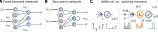
\includegraphics{media/chapters/02_modelling/02_02/neural_networks.pdf}%
	{\phantomsubcaption\label{fig:neural_networks_a}}%
	{\phantomsubcaption\label{fig:neural_networks_b}}%
	{\phantomsubcaption\label{fig:neural_networks_c}}%
	\caption[Illustration of different neural network types]{Illustration of different neural network types. Blue circles depict individual neurons. \textbf{(A)} Feed-forward neural networks can be represented as acyclic graphs. \textbf{(B)} If the network connectivity contains cycles (e.g., the 5-2-4-5 cycle), the network is called \emph{recurrent}. Cycles can also be self-recurrences (e.g., neuron 6). \textbf{(C)} Artifical neurons (\emph{left}) process time-discrete samples. Spiking neurons (\emph{right}) are time-continous; they receive a weighted input spike train, filter it, and produce an output spike train.}
\end{figure}

% How to build neural networks
% Define feed-forward and recurrent neural networks
% But how to select the weights?
% Solution that artificial neural networks do
% But is this what biology does?
% Rate vs temporal coding debate -> Aaron

We are now well-equipped to construct and simulate spiking neural networks (\SNNpl).
In theory, we just take $n$ spiking neurons and connect them up according to synaptic weights $w_{ij}$. As mentioned before, these weights determine the connection strength between a pre-neuron $j$ and post-neuron $i$. Inputs are additive over multiple pre-neurons (eqs.~\ref{eqn:low_pass_first_order}, \ref{eqn:low_pass_first_order_current}).%
\footnote{This notion of synaptic weights $w_{ij}$ assumes that each neuron possesses a single synaptic input channel.
Hence, there is only a single synaptic weight matrix.
For neurons with multiple synaptic input channels we can simply use an individual weight matrix for each input channel. We discuss this in the next chapter.}

Mathematically, the \emph{weight matrix} $\mat W \in \mathbb{R}^{n \times n}$ is the adjacency matrix of a directed connectivity graph.%
\footnote{For convenience and computational efficiency, neurons are typically grouped into \enquote{layers}, \enquote{populations}, or \enquote{ensembles} (all terms are used synonymously).
Not all layers have connections among each other. Hence, $\mat W$ typically is a block-matrix that can be split into multiple sub-matrices.}
Networks with acyclic connectivity are called \emph{feed-forward} (\Cref{fig:neural_networks_a}); networks with cyclic connectivity are \emph{recurrent} (\Cref{fig:neural_networks_b}).
Feed-forward \SNNpl have finite memory.
Assuming plausible synaptic filters, their impulse response decays exponentially.
In contrast, and as we discuss later, recurrent networks can posses more interesting dynamics.

To actually simulate an \SNN, we feed an external input (e.g., a set of currents or spike-trains) into the network and numerically integrate the coupled differential equations.
There are numerous general-purpose simulator software packages that do this efficiently, e.g., NEST \citep{gewaltig2007nest}, Brian \citep{stimberg2019brian}, GeNN \citep{yavuz2016genn}, or Nengo \citep{bekolay2014nengo}.

The most important question---and one that we pursue for the remainder of this thesis---is how to ultimately select $\mat W$.
For the artificial neural networks ({\ANN}s) used in machine learning (\Cref{fig:neural_networks_c}), the astoundingly successful answer is to use stochastic gradient descent on a loss function $E$, i.e., $\dot{\mat W} = -\eta \nabla_{\mat W} E(\vec a_k, \vec {\hat a_k})$, where $\eta$ is a learning rate, $\vec a_k$ is the desired output activity for an input sample $\vec x_k$, and $\vec{\hat a_k}$ is the actual output \citep{lecun2015deep}.
For example, one common choice for the loss function is $E(\vec a_k, \vec {\hat a_k}) = \|\vec a_k - \vec{\hat a}_k\|^2$.

Similar gradient-descent global optimisation methods can be applied in the context of \SNNpl as well.
\Citet{hunsberger2018spiking} characterises the \LIF response curve $G[J]$ in a network context and then trains an \ANN that uses $G[J]$ as a nonlinearity.
The resulting $\mat W$ can then be used in a spiking context.
\Citet{goltz2020fast} optimise synaptic weights such that desired spike-timings are generated by a black-box spiking neural network simulator.

%Computational neuroscientists often distinguish between rate and temporal spike-codes, though the definitions of these concepts are quite vague.
%For example, \citet[Chapter~1]{gerstner2002spiking} list three different definitions of the term \enquote{rate code}, while \citet{abbott2001theoretical} list four definitions.
%Rates are estimated by either binning and counting, causal and acausal filtering, or (orthogonally) taking averages over entire populations into account.

%A similar zoo of definitions is to be had for temporal codes. For example, as pointed out by \citet[Chapter~14]{koch1999biophysics}, researchers often interpret temporal codes as correlations between spike times carrying information (i.e., spikes from different pre-neurons arriving earlier or later relative to each other).
%Another popular temporal code is \enquote{time-to-first-spike}, i.e., the notion that neurons rely on the time between some synchronisation event and the first received spike event \citep{vanrullen2005spike}.

Notably, such global optimisation methods can be useful when modelling neurobiological systems.
For example, there are striking similarities between the neural tuning observed in visual cortex and the learned tuning of neurons in hierarchical image classification networks \citep{yamins2016using}.
However, this is, to some degree, accidental, and not explicitly imposed.
As we discussed at the beginning of this chapter, it is desirable build models that reliably adhere to certain constraints---such as the aforementioned tuning properties.

\subsection{Neural Tuning and Population Codes}
\label{sec:neural_tuning}

\begin{figure}
	\centering
	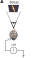
\includegraphics{media/chapters/02_modelling/02_02/visual_cortex_tuning_setup.pdf}%
	\includegraphics{media/chapters/02_modelling/02_02/visual_cortex_tuning.pdf}
	\caption[Neural tuning in the visual cortex]{Neural tuning in the visual cortex.
	\textbf{(A)} Illustration of the original experiment by \citet{hubel1959receptive}. Bright rectangles are briefly presented on a dark screen to an animal while recording from a neuron in its visual cortex. \textbf{(B)} Recorded spike trains for different stimulus orientations. Horizontal lines are the stimulus presentation interval. Adapted from \citet[Figure~3]{hubel1959receptive}. \textbf{(C)} The mapping between stimulus $\vec x$ and activity $a$ forms a \emph{tuning curve}. This neuron is tuned to vertical bars.}
	\label{fig:visual_cortex_tuning}
\end{figure}

%Given that we can simulate large biological systems at different levels of abstraction, the primary challenge is to construct networks that actually give rise to the behaviours observed in nature.
%Unfortunately, in many cases, too much about the brain is still unknown to successfully build such models.
%This is particularly true for brain regions involved in higher level cognition, and that, in terms of connectivity, are farther away from the periphery.
%Fortunately, brain regions \emph{closer} to the periphery are, relatively speaking, quite well understood.
%\footnote{Neuroscience textbooks such as \citet{kandel2012principles} discuss the neural circuitry of brain regions involved in sensory and motor processing in great detail, while chapters concerning higher-level cognitive tasks mostly report behavioural observations and coarse measurements such as fMRI scans.}
There are two important concepts that shed some light onto the organisation of brain networks---at least those brain networks involved in sensory processing: \emph{tuning curves} and \emph{receptive fields}.
In turn, these ideas motivate \emph{population codes}, which we heavily rely on in the context of our modelling tool, the Neural Engineering Framework---we discuss this in the next section.

\subsubsection{Tuning curves}
%Early studies on these concepts were conducted by \citeauthor{hubel1959receptive}.
In a famous \citeyear{hubel1959receptive} experiment (cf.~\Cref{fig:visual_cortex_tuning}), Hubel and Wiesel present a visual stimulus in the form of a bright rectangle at different orientations $\varphi$ to an experimental animal.
At the same time, the activity of a neuron in the animal's visual cortex is recorded.
This characterizes how the stimulus propagates through the brain up to the recording site.
%We characterize neurons in terms of their own physiological properties \emph{and} in terms of the preceding network connectivity.

In the recording depicted in \Cref{fig:visual_cortex_tuning}, we find that the neuron is most sensitive to---or, \emph{tuned} to---a certain orientation $\varphi$.
We could say that in this specific case, vertical bars are the \emph{preferred stimulus} of the neuron.
Generally, such a mapping from a stimulus property $\varphi$ onto the average neural activity $a(\varphi)$ is called a \emph{tuning curve} \citep[e.g.,][p.~1112]{vandenbos2015apa}.

\subsubsection{Receptive fields}

\begin{figure}
	\centering
	\includegraphics{media/chapters/02_modelling/02_02/gabor_filters.pdf}
	\caption[Examples of randomly generated of Gabor filters]{Examples of randomly generated Gabor filters.
	Each filter is a two-dimensional function $e(\xi_1, \xi_2)$, where $(\xi_1, \xi_2)$ is a spatial location.
	Negative  values (red) indicate that neural activity is reduced if a stimulus is present at that location, positive values (blue) indicate an increase in activity.}
	\label{fig:gabor}
\end{figure}
The concept of \emph{receptive fields} is closely related to tuning curves.
This is best illustrated in the context of stimuli that can be described as an intensity over a two-dimensional surface---such as vision or touch.
Generally, the receptive field of a neuron is the collection of points $(\xi_1, \xi_2)$ at which the presence of a stimulus---a point of light or mechanical pressure---triggers a neural response.
However, as evidenced by \citet{hubel1962receptive}, neural receptive fields are not only characterised in terms of the locations where a stimulus \emph{increases} the average neural activity, but also where the presence of a stimulus \emph{decreases} activity.

Mathematically, we can describe this in terms of a function $e(\xi_1, \xi_2)$ that assigns a weight to each stimulus location $(\xi_1, \xi_2)$.
This function $e$ is the receptive field.
\emph{Gabor filters} are a class of mathematical functions that fit observed receptive fields in the visual cortex well \citep{marcelja1980mathematical,field1986structure}.%
\footnote{Gabor filters are sinusoidals scaled by a radial Gaussian envelope. Such functions are maximally localised in time and space, as pointed out in the context of Gabor's Fourier uncertainty principle \citep{gabor1946theory}.}
Examples are depicted in \Cref{fig:gabor}.

Borrowing some notation from the next section, the activity of the neuron $a(x)$ can be modelled as the product between the receptive field $e$ and the stimulus $x$ integrated over space (where $x(\xi_1, \xi_2)$ is a function describing the stimulus intensity at a certain location)
\begin{align}
	a(x) &= G\left[ \alpha \iint e(\xi_1, \xi_2) x(\xi_1, \xi_2) \,\mathrm{d}\xi_1\mathrm{d}\xi_2 + \beta \right]
		= G \bigl[ \alpha \langle e, x \rangle + \beta \bigr] \,.
	\label{eqn:tuning_curve_from_receptive_field}
\end{align}
Here, $\langle e, x \rangle$ is the inner product between the receptive field and the stimulus (see \Cref{app:functional_analysis} for an introduction to functional analysis and the corresponding definitions).
Furthermore, $G$ is a rate approximation of the neuron model (see previous subsection), and, $\alpha > 0$ and $\beta$ translate the inner product into a neural input current.

Importantly, if the stimulus and receptive field are normalised, then $\langle e, x \rangle$ is the cosine similarity between the two functions.
Correspondingly, according to the above model, the neural response is maximised if $e = x$.
In other words, the receptive field \emph{is} the \enquote{true} preferred stimulus of a neuron.
This is consistent with modern definitions of the term \enquote{receptive field} in the neuroscience literature \citep[cf.][]{troy2009retinal}.

\begin{figure}
	\centering
	\includegraphics{media/chapters/02_modelling/02_02/visual_cortex_receptive_field_example.pdf}
	\caption[Model of the Hubel and Wiesel experiment]{Model of the original Hubel and Wiesel experiment (cf.~\Cref{fig:visual_cortex_tuning}). \textbf{(A)} The receptive field $e(\xi_1, \xi_2)$ describes whether a stimulus location $(\xi_1, \xi_2)$ acts excitatory (blue), or inhibitory (red). \textbf{(B)} The stimulus is a light rectangle at different orientations $\varphi$; this can be described as a function $x$ mapping locations onto light intensity. \textbf{(C)} Tuning curve obtained according to the model in \cref{eqn:tuning_curve_from_receptive_field}.}
	\label{fig:visual_cortex_receptive_field_example}
\end{figure}

\Cref{fig:visual_cortex_receptive_field_example} illustrates the relationship between the receptive field of a neuron and one of its tuning curves.
Choosing a vertically oriented Gabor filter as a receptive field, we can model the orientation tuning from the original Hubel and Wiesel experiment.
Thus, in a nutshell, a tuning curve is a characterisation of the neuron in terms of a specific stimulus property (e.g., the orientation of a bar of light), whereas the receptive field models its tuning properties in general (e.g., the predicted activity for any visual stimulus).

\subsubsection{Population codes}
Although tuning curves and receptive fields are inherently reconstructed from a network context, they still only characterise individual neurons.
To better understand biological neural networks, we need to consider the tuning properties of groups of neurons.

Doing this, we find that neighbouring neurons often have similar tuning properties---they are tuned to the same sensory modality, and possess similar receptive fields \citep{berkowitz2009population}.
Again, this has been explored well in context of orientation tuning in the visual cortex \citep[Chapter~25]{kandel2012principles}.
For example, neurons in visual cortex are organised in \enquote{cortical columns}.
Each column consists of several layers of neurons.
Within a single layer of the same column, neurons possess the similar preferred orientations.
Between columns, preferred orientations differ significantly.

This, as well as several other observations \citep{yuste2015neuron}, suggest that brain networks use \emph{population codes}.
The idea is that a single underlying quantity---such as the orientation of a visual stimulus---is represented by a group of neurons in a distributed manner.
The opposite would be \enquote{single-neuron coding}, where the activity of individual, localised neurons maps onto some quantity, or, in higher-level cognition, onto specific concepts \citep{berkowitz2009population}.

\begin{figure}
	\centering
	\includegraphics{media/chapters/02_modelling/02_02/population_code.pdf}
	\caption[Probabilistic decoding of scalar quantities using population codes]{Probabilistic decoding of scalar quantities using population codes.
	\textbf{(A)} \emph{Left:} The activity $a$ of a single neuron represents a scalar value $x \in [-1, 1]$.
	The current $J$ fed into each neuron is subject to Gaussian noise with standard deviation $\sigma = \SI{1}{\nano\ampere}$.
	Solid line corresponds to the median activity for the given represented value; shaded area corresponds to a contour line of the underlying probability density.
	\emph{Right:} Trying to decode the represented value $x$ from the activity results in significant uncertainties; negative values cannot be disambiguated. Dotted line is the optimum; solid line the median of a maximum-likelihood estimate, shaded area a contour line of the underlying probability density.
	Error $E$ is the decoding \RMSE.
	\textbf{(B, C, D)} The larger the number of neurons, the smaller the uncertainties.}
	\label{fig:population_code}
\end{figure}

Population codes are intriguing as a model for representation in biological networks.
They allow precise inferences from imprecise or ambiguous observations. This is illustrated in \Cref{fig:population_code}.
For example, we can imagine that a single neuron represents a scalar value $x \in [-1, 1]$ as expressed by its tuning curve $a(x)$.
Unfortunately, the firing rate $a$ cannot be measured without error.
That is, neurons produce spontaneous activity that, as far as we can tell, is not related to a stimulus.
This is part due to noise inherent to neurobiological processes \citep[cf.][Section~2.2.1]{eliasmith2003neural}, and in part due to the Fourier uncertainty principle.%
\footnote{We can either estimate the frequency (i.e., rate) of a signal with a high precision at a low temporal resolution, or estimate the frequency with a low precision at a high temporal resolution \citep{gabor1946theory}.}
Hence, when trying to \emph{decode} the represented value $x$ from the neural activity, there is a large degree of uncertainty.
Adding neurons that are tuned to the same quantity $x$, but with different tuning curves to the population drastically reduces this uncertainty from a information-theoretic perspective \citep{ma2009population}.


\clearpage
\setcounter{section}{2}
% !TeX spellcheck = en_GB

\section{The Neural Engineering Framework}
\label{sec:nef}

\begin{figure}[p]
	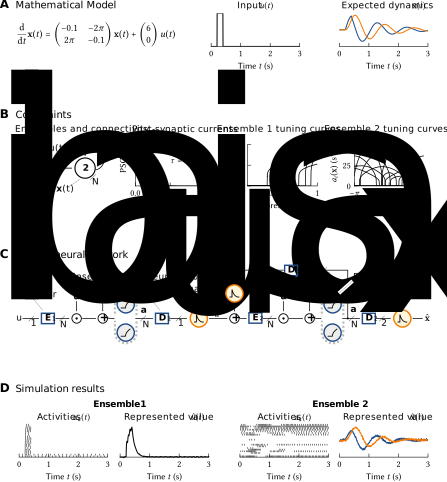
\includegraphics{media/chapters/02_modelling/02_03/nef_overview.pdf}
	\caption[Overview of the Neural Engineering Framework]{Overview of the Neural Engineering Framework (\NEF).
	\textbf{(A,~B)} Researchers provide a mathematical model or sampled data (sampled data shown here are random and only for illustration purposes), as well as a set of constraints.
	In this example, constraints are the overall connectivity, tuning properties and filter properties of post-synaptic currents. $\angle \vec x$ denotes the angle of $\vec x = (x_1, x_2)$, i.e., $\angle \vec x = \mathrm{arctan2}(x_2, x_1)$. \textbf{(C)} The \NEF can be used to systematically construct a spiking neural network from the given data. This network optimally implements the mathematical model under the given constraints.
	\textbf{(D)} Simulating the network gives insights into how well the mathematical description can be implemented on a neural substrate.
	Spike raster plots with neural activity depict output spikes (short vertical lines) for each neuron (corresponding to rows) over time.}
	\label{fig:nef_overview}
\end{figure}

As we mentioned at the beginning of this chapter, the Neural Engineering Framework (\NEF; \cite{eliasmith2003neural}) is a modelling framework for neurobiological systems.
The \NEF combines techniques from engineering and mathematics---particularly control and dynamical systems theory---with the neurobiological concepts discussed before.
The goal is to allow researchers to map high-level descriptions of cognitive phenomena onto low-level spiking neural networks.
As such, the \NEF provides a synthesis of bottom-up and top-down modelling, and is an attempt at a theory of neuroscience that spans multiple levels of analysis.

To use the \NEF, researchers systematically apply three \enquote{principles} that encapsulate key assumptions about neurobiological systems.
These principles exploit neural nonlinearities and synaptic filters to describe how vectorial quantities can be represented, transformed, and made to follow certain dynamics in a spiking neural fabric.
The resulting neural networks adhere to mechanistic constraints, such as neural connectivity, maximum firing rates, tuning properties, and synaptic time-constants.
This is illustrated schematically in \Cref{fig:nef_overview}.
A software tool that automates the process of translating mathematical models into spiking neural networks using the \NEF principles is part of the Nengo spiking neural network simulator package \citep{bekolay2014nengo}.\footnote{See \url{https://www.nengo.ai/} for more information on Nengo. Nengo is free for non-commercial use.}


%\begin{enumerate}[1.]
%	\item \emph{Representation.}
%	The momentary activity $\vec a \in \mathbb{R}^{\Npop}$ of an ensemble of \Npop neurons represents a vectorial quantity $\vec x \in \mathbb{R}^d$. The encoding process mapping $\vec x$ onto activities $\vec a$ is nonlinear,
%	the decoding process is linear.
%	That is, there exists a matrix $\Dec \in \mathbb{R}^{d \times \Npop}$ such that $\vec x \approx \vec \Dec \vec a(\vec x)$.
%	\item \emph{Transformation.}
%	Synaptic connections between neural ensembles approximate nonlinear transformations $f(\vec x)$ applied to the represented values, where $f : \mathbb{R}^d \longrightarrow \mathbb{R}^{d'}$ and $d$ and $d'$ are the dimensionalities of the quantities represented in the individual ensembles.
%	\item \emph{Dynamics.}
%	Represented values are state variables $\vec x(t)$ in a dynamical system. Recurrent connections approximate arbitrary dynamical systems of the form $\dot{\vec x} = f(\vec x(t), \vec u(t), t)$.
%	Here, $\vec x(t)$ is the represented value, $\vec u(t)$ is some external input, and $t$ is the current time.
%\end{enumerate}

In this section, we first discuss applications of the \NEF from the perspective of the cognitive sciences (model validation and hypothesis generation), as well as engineering and computer science (a programming model for neuromorphics).
We continue with a detailed description of the theory underpinning the \NEF, and conclude with a list of limitations that we address in the next chapters.

\subsection{Model Validation and Hypothesis Generation}
\label{sec:nef_purpose}

As we alluded to in the introduction of this chapter, models built using the \NEF bridge multiple levels of analysis.
That is, they implement high-level behaviour (given as a mathematical description) using low-level mechanisms (spiking neurons and synapses).
This facilitates model validation and hypothesis generation.

\subsubsection{Model validation}
The concept of model validation generally refers to comparing a model to empirical measurements \citep{adams2012assessing}.
In the case of \NEF models, we can, of course, compare the high-level behaviour of the biological system to that of the constrained network model.
The smaller the deviations, the \enquote{better} the original mathematical model.%
\footnote{Of course, naively evaluating models in this manner does not account for overfitting. The model could inadvertently be tuned to reproduce the behaviour of interest, but not be able to generalise to different scenarios. In contrast to other machine learning approaches, overfitting in this sense is typically less of a problem with \NEF models.
This is due to the transparency of the training process, only few (typically hand-selected) parameters, and biological constraints, all of which can be seen as regularisation.}
While such comparisons would also be possible with the high-level model alone, biological constraints can drastically influence the high-level behaviour of the model.
The \NEF is thus a good litmus test for the suitability of a mathematical model to be realised on a neural substrate.
This is because the \NEF \emph{optimally} implements a set of mathematical equations as an idealised spiking neural network.
If the model cannot be realised on a spiking neural substrate despite these idealised conditions, it is unlikely that it describes a biological process well.

\NEF models can also be compared in terms of detailed neurophysiological data, and not just high-level behaviour.
Because \NEF models are based on a biologically plausible neural substrate, researchers can measure neurophysiological quantities, such as spike trains, local field potentials, or blood oxy\-gen\-ation \citep[Chapters 5.8~\&~9.4]{eliasmith2013how}.
Examples of this can be found in \citet{stewart2012learning,bekolay2014spiking,duggins2017effects,voelker2018improving,gosmann2021cue}.

\subsubsection{Hypothesis generation}
There are two ways in which the \NEF aids \emph{hypothesis generation}.
First, and closely related to model validation, deviations between the constrained simulation and the original mathematical model may indicate that the high-level description cannot be realised by the biological system.
Hence, the \NEF can be used to reject unsuitable hypotheses and to guide theories towards higher degrees of biological plausibility.
Examples of cognitive theories developed in conjunction with the \NEF include the Semantic Pointer Architecture (SPA; \cite{eliasmith2013how}) and SPAUN (the \enquote{Semantic Pointer Architecture Unified Network}), a functional brain model capable of a variety of cognitive tasks \citep{eliasmith2012largescale}.

Second, \NEF models can be used to predict the behaviour of a system in experimental paradigms for which no empirical data exists (yet).
This prediction then forms a hypothesis that can be compared to future empirical data.
Furthermore, the \NEF also enables the systematic variation of observed biological parameters (e.g., time-constants or connectivity), which is often not easily possible in real biological systems.
Assessing the system performance in such artificial situations may yield hypotheses as for why evolution favoured certain parameter combinations.
We give an example of this in \Cref{chp:cerebellum}.

\subsection{Applications to Neuromorphic Computing}
\label{sec:neuromorphic}

The scientific applications discussed above were the primary motivation for the development of the \NEF.
However, coincidentally, the same methods are useful as a programming model for neuromorphic computers \citep{boahen2017neuromorph,voelker2021programming}.

\subsubsection{Neuromorphic computers}
Coined by \citet{mead1990neuromorphic}, this term refers to computer systems that---to some degree---mimic information processing in the brain.
This typically implies numerous simple computational units, \emph{neurons}, connected via a flexible interconnect \citep{furber2016largescale}.
Beyond these basic characteristics there is no consensus as for what exactly constitutes a \enquote{neuromorphic computer}.
However, most neuromorphic hardware systems execute computations asynchronously and possess provisions for sparse event-based signalling.
Akin to biology, individual computational units independently generate binary events.
In contrast to artificial neural networks, computation is inherently temporal; communication occurs sporadically and does not carry continuous values.
Hence, the underlying communication infrastructure solely carries temporally sparse spike events, minimising the amount of transferred data.

Current neuromorphic computers can be roughly split into two categories, depending on the specific realisation of the computing elements.
Computation either takes place in analogue model circuits, similar to the \LIF circuit (\Cref{fig:lif}), or digital processors with varying degrees of programmability.
Examples of systems in the former \enquote{mixed-signal} category include Braindrop \citep{neckar2019braindrop} and BrainScaleS \citep{schemmel2010waferscale}.
Systems that fall into the latter \enquote{purely digital} category are SpiNNaker \citep{furber2013overview} and Loihi \citep{davies2018loihi}. See \citet{furber2016largescale} for a more comprehensive list.

\subsubsection{Applications of neuromorphic computing}
The primary motivation behind neuromorphic hardware is to construct computing hardware that approaches the energy efficiency of biological brains \citep{mead1990neuromorphic,boahen2017neuromorph}.
Compared to conventional computer architectures, these energy savings are mostly due to the asynchronous nature of the computational units, as well as the reduction in communication bandwidth due to event-based signalling \citep{painkras2013spinnaker}.
Furthermore, mixed-signal neuromorphic computers with analogue model circuits benefit from each computational unit operating close to the theoretically required minimum energy \citep{boahen2017neuromorph}.
However, compared to purely digital systems, such analogue designs are much more challenging to build from an engineering perspective.

Being able to reliably simulate large spiking neural networks with a low energy footprint would be a major scientific breakthrough.
For example, this would enable large-scale brain simulations that are infeasible with conventional supercomputers \citep{calimera2013human}.
From an engineering perspective, being able to map artificial neural networks onto neuromorphic computers could greatly reduce energy costs of machine learning in the data centre and enable new mobile applications of artificial intelligence \citep{hunsberger2016training,blouw2018benchmarking,goltz2021fast,blouw2020eventdriven}.
Due to the inherent temporal aspect of the computation, spiking neural networks and neuromorphic hardware are particularly well-suited for applications requiring real-time stream processing, such as robotic control or autonomous drones \citep{komer2015biologically,yan2021comparing}.

\subsubsection{The \NEF as a programming model for neuromorphic computers}
While, as of writing, several neuromorphic hardware platforms are available to the wider research community, a remaining challenge is to actually program these systems.
Since the computational fabric of neuromorphic computers is similar to biological neural substrates, the \NEF can be used to translate mathematical descriptions of dynamical systems into network models that can be executed on the hardware system \citep{boahen2017neuromorph}.
The given constraints can be used to reflect the capabilities of the hardware and to specify the desired precision of the computation.
A variety of neuromorphic platforms have been included as an execution target in Nengo, catering to both scientific and engineering applications.

\pagebreak

\subsection{Principle 1: Representation}

\label{sec:nef_representation}

As we saw above, the Neural Engineering Framework has useful applications in both science and engineering.
In the first part of this thesis, we discuss extensions to the \NEF that allow us to model neurobiological circuits more accurately and to take better advantage of the computational resources found on neuromorphic computers.
In preparation for these extensions, we now provide a detailed discussion of the aforementioned \enquote{three principles} at the core of the \NEF.

The first two \NEF principles are best explained assuming steady-state average activities, although, as mentioned before, biological neural networks inherently form dynamical systems.
However, our use of average rate approximations should not be interpreted as the adoption of a \enquote{rate code} by the \NEF, but, as we discuss below, is a convenience for solving the synaptic weight optimisation problem.
All optimisations can be done in the spiking domain, but the computational costs are significantly higher~\citep{macneil2011finetuning}.

For now, our goal is to map static equations of the form $\vec y = f(\vec x)$ onto rate approximations of spiking neural networks.
The first \NEF principle describes how neuron populations represent quantities such as $\vec x$ and $\vec y$.
Paraphrasing \citet{eliasmith2003neural}:
\begin{framed}
\noindent\emph{\NEF Principle 1.}
The momentary activity $\vec a \in \mathbb{R}^{\Npop}$ of a population of \Npop neurons represents a vectorial quantity $\vec x \in \mathbb{R}^d$. The encoding process mapping $\vec x$ onto activities $\vec a$ is nonlinear,	the decoding process is linear.
That is, there exists a matrix $\Dec \in \mathbb{R}^{d \times \Npop}$ such that $\vec x \approx \vec \Dec \vec a(\vec x)$.
\end{framed}
There are two fundamental assumptions in this principle that deserve to be untangled.
First, we assume that neuron \emph{populations} form basic functional units and, second, that biological systems represent vectorial quantities.
We already discussed the first assumption regarding populations in more detail in \Cref{sec:neural_tuning}.
To summarise, neighbouring neurons are sensitive to the same quantity and neural activities are noisy---this suggests that nervous systems use population codes.
The second assumption deserves more explanation, given that vectors are abstract mathematical objects.

\subsubsection{Vectorial representations}
The assumption that populations represent vectors $\vec x \in \mathbb{R}^d$ is---to some degree---a mathematical convenience.
Many mathematical objects have useful equivalent vectorial representations, including functions \citep[Chapter 3]{eliasmith2003neural}, probability densities \citep[Chapter 9]{eliasmith2003neural}, and symbols (via vector symbolic architectures; see \cite{gayler2003vector}, \cite{eliasmith2012largescale} and \cite{eliasmith2013how}).
% TODO: Reference review of function spaces

Additionally, there is strong evidence that the activities of neural populations form smooth low-dimensional manifolds in a high-dimensional activity space \citep{gallego2017neural,stringer2019highdimensional}.
There exists a mapping $\vec a: \mathbb{R}^d \longrightarrow \mathbb{R}^{\Npop}$ (with $d \ll \Npop$) between a low-dimensional vector $\vec x \in \mathbb{R}^d$ and the average neural activities $\vec a(\vec x) \in \mathbb{R}^{\Npop}$, where \Npop is the number of neurons in the population.
If the population exhibits activities $\vec a(\vec x)$ associated with a value $\vec x$, then the population \emph{represents} a \Ndim-dimensional quantity $\vec x$.

\subsubsection{Encoding vectorial quantities}

\begin{figure}
	\centering
	\includegraphics{media/chapters/02_modelling/02_03/nef_representation_2d.pdf}
	{\phantomsubcaption\label{fig:nef_representation_2d_surface}}
	{\phantomsubcaption\label{fig:nef_representation_2d_unit_circle}}
	\caption[Obtaining bell-shaped tuning curves when using two-dimensional encoders]{Obtaining bell-shaped tuning curves when using two-dimensional encoders. Figure adapted from \citet[Figure~2.8, p.~52]{eliasmith2003neural}.
	\textbf{(A)} The surface plot of the tuning curve of a single neuron. The orange arrow points in the direction of the encoder $\vec e_i$.
	\textbf{(B)} The tuning curve for a represented value $\vec x$ of constant magnitude over the angle $\angle \vec x$.
	The orange triangle corresponds to the direction of the encoder.
	The neuron is most active for represented values pointing in this direction.
	}
	\label{fig:nef_representation_2d}
\end{figure}

As we have discussed in \Cref{sec:neural_tuning}, the relationship between a stimulus $\vec x$ and activities of an individual neuron are also referred to as a \enquote{tuning curve}.
While tuning curves in neuroscience are typically defined over scalar quantities, \citeauthor{eliasmith2003neural} propose a parametrised encoding equation $a_i(\vec x)$ that maps $\vec x \in \mathbb{R}^{\Ndim}$ onto the activities of the $i$th neuron in a population---similar to the mathematical model we presented to describe tuning curves in the Hubel and Wiesel experiment (\Cref{sec:neural_tuning},  \Cref{fig:visual_cortex_receptive_field_example} and eq.~\ref{eqn:tuning_curve_from_receptive_field}):
\begin{align}
a_i(\vec x) = G\big[J_i\big(\langle \vec x, \vec e_i \rangle\big)\big] = G\big[\alpha_i\langle \vec x, \vec e_i \rangle + \beta_i\big] \,,
 \quad\quad \text{where } i \in \{1, \ldots, N\} \,.\label{eqn:encoding}
\end{align}
Depending on the interpretation, the encoding vector $\vec e_i$ is equivalent to the \enquote{receptive field} or \enquote{preferred direction} of the neuron.
For example, as depicted in \Cref{fig:nef_representation_2d}, a two-dimensional encoding vector can be used to construct bell-shaped tuning curves similar to those discussed in the context of orientation tuning in the visual cortex; here, the vector $\vec e_i$ would stand for a preferred direction.
Of course, $\vec e_i$ and $\vec x$ could also be discretised visual stimuli---in this case, $\vec e_i$ would be a receptive field and \cref{eqn:encoding} is a discrete approximation of \cref{eqn:tuning_curve_from_receptive_field}.

The response curve $G[J]$ depends on the underlying neuron model; for example, we derived the response curve for \LIF neurons in \Cref{sec:simplified_neuron_models} (eq.~\ref{eqn:lif_response_curve}); 
the current translation function $J_i(\xi)$ is typically an affine mapping parametrised by a gain $\alpha_i$ and a bias current $\beta_i$.

When building \NEF systems, modellers choose the parameters of $a_i(\vec x)$ to characterise how a stimulus $\vec x$ \emph{should} be reflected in the activities of individual neurons.
This last emphasis on \emph{should} is important.
Modellers establish a \emph{normative constraint}.
They specify what the desired tuning should \emph{optimally} be---for example, taking biological data into account.
The purpose of the \NEF is to ensure that this constraint is met in a network context.


\begin{figure}
	\centering
	\hspace{-0.2cm}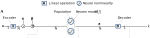
\includegraphics{media/chapters/02_modelling/02_03/nef_representation_diagram.pdf}
	\includegraphics{media/chapters/02_modelling/02_03/nef_representation.pdf}
	{\phantomsubcaption\label{fig:nef_representation_diagram}}
	{\phantomsubcaption\label{fig:nef_representation_current_translation}}
	{\phantomsubcaption\label{fig:nef_representation_tuning_curves}}
	{\phantomsubcaption\label{fig:nef_representation_deocding}}
	\caption[Representation in the Neural Engineering Framework]{Representation in the Neural Engineering Framework. Example for a population of $N = 10$ neurons representing a one-dimensional quantity.
	\textbf{(A)} Schematic overview of the encoding and decoding process.
	\textbf{(B)} Randomly selected affine current translation functions $J_i(\xi) = \alpha_i \langle \vec x, \vec e_i \rangle + J^\mathrm{bias}_i$. The dotted line corresponds to the activity threshold $J_\mathrm{th}$.
	\textbf{(C)} Tuning curves for each neuron in the population after applying the somatic nonlinearity $G[J]$~(eq.~\ref{eqn:lif_response_curve}).
	\textbf{(D)} Reconstructing the represented value from neuron activity by means of linear decoding. Dashed line corresponds to the ideal.}
	\label{fig:nef_representation}
\end{figure}

\subsubsection{Selecting encoders, gains, and biases}
Of course, this raises the question of how modellers should select encoders $\vec e_i$, biases $\beta_i$, and gains $\alpha_i$.
To form a good basis for a population code, the population must exhibit diverse tuning (cf.~\Cref{fig:population_code}).
At the same time, the tuning curves must stay within modelling constraints such as the maximally observed firing rates $a_i$ for the range of stimuli $\vec x$ over which we characterise the neuron population.
We denote the set of represented values as a compact set \Xrepr with finite, non-zero volume $\vol(\Xrepr)$.

Unless more specific data are available, we can for example assume that $\vec x$ are within a hyperball of radius $r$, i.e., $\Xrepr = r \Ball^d$.
The encoding vectors $\vec e_i$ can be sampled from the unit hypersphere $\mathbb{S}^d$.
For monotone increasing response curves $G$, gain $\alpha$ and bias $\beta$ can be computed for each neuron by sampling an \enquote{$x$-intercept} value $\xi_0$ from the interval $[-r, r]$ and a maximum rate $a_\mathrm{max}$.
We then solve for $\alpha$, $\beta$ such that the following equations hold:
\begin{align*}
	\alpha \xi_0 + \beta &= J_0 = G^{-1}[0] \,, &
	\alpha r + \beta &= J_\mathrm{max} = G^{-1}[a_\mathrm{max}] \,, & \text{where } G^{-1}[a] &\coloneqq \max \big\{ J \mid G[J] = a \big\} \,.
\end{align*}
We get $(r - \xi_0) \alpha = J_\mathrm{max} - J_0$, $(r - \xi_0) \beta = (r J_0 - \xi_0 J_\mathrm{max})$.
For example, for each tuning curve in \Cref{fig:nef_representation}, we randomly sampled a $\xi_0$ from a uniform distribution over $[-1, 1]$, and a maximum firing $a_\mathrm{max}$ rate uniformly from $[10, 50]$.

\subsubsection{Computing identity decoders}
\Cref{eqn:encoding} describes the average neural activities $\vec a$ we expect when a population is representing a certain value $\vec x$; that is, this equation describes how quantities $\vec x$ are \emph{encoded} in a neural network.
Complementary to encoding is \emph{decoding}.
That is, given the activities $\vec a$, we would like to reconstruct the represented $\vec x$.
This could---for example---be accomplished using Bayesian inference, as we demonstrated in \Cref{fig:population_code}.
If the number of neurons \Npop in a population is large enough we can, to a very similar effect, just use a linear decoding matrix \Dec (\Cref{fig:nef_representation}; \cite{salinas1994vector}).

The idea is to simply multiply the activities $\vec a$ with a matrix $\Dec \in \mathbb{R}^{d \times \Npop}$ such that the decoded $\vec{\hat x} = \Dec \vec a(\vec x)$ is approximately equal to the encoded $\vec x$, for any $\vec x \in \Xrepr$.
Under the assumption that the activities $\vec a$ are subject to independent and identically distributed (i.i.d.) zero-mean Gaussian noise with standard-deviation $\sigma$, the decoding matrix \Dec can be obtained by minimising a least-squares loss-function $E$:
\begin{align}
	E &= \frac{1}{\vol(\Xrepr)} \iint_{\Xrepr} \bigl\| \vec x - \Dec \bigl( \vec a(\vec x) + \nu \bigr) \bigr\|_2^2  \, \mathrm{d}\vec{x} \quad\quad \text{where } \nu \sim \Normal(0, \sigma) \,.
	\label{eqn:lstsq_loss_identity}
\end{align}
Of course, minimising this integral directly is infeasible.
We approximate a solution numerically by drawing \Nsmpls samples from \Xrepr, denoted $\vec x_1$, $\ldots$, $\vec x_N$.
Arranging the samples and the corresponding population activities in matrices $\mat X = \begin{pmatrix} \vec x_1, \ldots, \vec x_{\Nsmpls} \end{pmatrix} \in \mathbb{R}^{\Nsmpls \times \Ndim}$ and $\mat A = \begin{pmatrix}\vec a(\vec x_1), \ldots, \vec a(\vec x_{\Nsmpls})\end{pmatrix} \in \mathbb{R}^{\Nsmpls \times \Npop}$, we can phrase finding \Dec as a Tikhonov regularised least-squares optimisation problem
\begin{align}
\min_{\Dec} \sum_{k = 1}^{\Nsmpls} \| \Dec \vec a(\vec x_k) - \vec x_k \|_2^2  + \| \sigma \Dec \|^2_\mathrm{F}
&= \min_{\Dec} \| \mat A \Dec^T - \mat X \|_\mathrm{F}^2 + \sigma^2 \Nsmpls \| \Dec \|_\mathrm{F}^2 \,,
\label{eqn:lstsq_loss}
\end{align}
where $\lambda = N \sigma^2$ is the regularisation factor.
From a probabilistic perspective, this particular choice of $\lambda$ results in the exact maximum a-posteriori solution for $\mat D$ with the prior assumption that there is Gaussian noise with standard deviation $\sigma$ on the measurements $\mat A$ \citep[Chapter~6]{boyd2004convex}. 
Larger $\lambda$ increase the robustness of the solution with respect to noise, but decrease the noise-free approximation error.
The solution can be expressed in terms of the regularised Moore-Penrose pseudo-inverse:
\begin{align}
\Dec^T &= \mat A^+ \mat X \,, &\text{where} \quad \mat A^+ &= \bigl(\mat A^T \mat A + \lambda N \mat I \bigr)^{-1} \mat A^T \,.
\label{eqn:decoding}
\end{align}
As explored by \citet[Chapter~2]{eliasmith2003neural}, the decoding error $E$ tends to decrease with $\mathcal{O}(\sqrt{n})$, assuming that the tuning curves have uniform $x$-intercepts and random encoders $\vec e_i$.
An example of this decoding scheme is given in \Cref{fig:nef_representation_deocding}.

Note that, as mentioned before, we do not take dynamics into account when computing the decoders \Dec.
However, as we discuss next, the same \Dec can be used to decode represented values through time in spiking networks when defining activity $\vec a(t)$ as low-pass filtered population spike trains.
We explicitly take temporal aspects of neural computation into account in \Cref{sec:nef_dynamics} below, and when we discuss temporal tuning in Chapter~4.

\pagebreak

\subsection{Principle 2: Transformation}
\label{sec:nef_transformation}

The representation principle maps vectors $\vec x$ onto average neural activities $\vec a(\vec x)$.
Of course, individual neuron populations seldom exist in isolation.
To construct \emph{networks} that realise the desired tuning properties, we need to determine synaptic weights $w_{ij}$ that describe the connection strength between the $j$th pre- and the $i$th post-neuron.
In addition to realising the chosen representations, the \NEF puts a further modelling constraint on the synaptic weights:
\begin{framed}
\noindent\emph{\NEF Principle 2.} Synaptic connections between neural ensembles approximate nonlinear transformations $\vec y = f(\vec x)$, where $\vec x \in \mathbb{R}^d$ is the value represented in the pre-population, and $\vec y \in \mathbb{R}^{d'}$ the value represented in the post-population.
\end{framed}

\begin{figure}
	\centering
	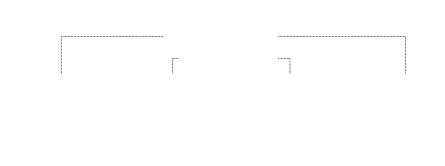
\includegraphics{media/chapters/02_modelling/02_03/nef_transformation_annotations.pdf}%
	\kern-157.19mm\includegraphics{media/chapters/02_modelling/02_03/nef_transformation.pdf}
	\caption[Examples of the function decoding scheme]{Examples of the function decoding scheme. Instead of decoding the represented value $\vec x$ from a neuron population, we can approximate arbitrary functions $f(\vec x)$.
	\textbf{(A)} $\Npop = 20$ tuning curves $\vec a(x)$; same parameters as in \Cref{sec:nef_representation}. \textbf{(B-E)} Different linear decodings $\mat D^f \vec a(x)$ of the above tuning curves. Dotted line is the target function, thick line the decoded function. Inset $E$ is the \RMSE.
	}
	\label{fig:nef_transformation}
\end{figure}

That is, modellers can choose a transformation $f$ that should be computed in a connection.
We can easily approximate functions $f$ of the value $\vec x$ represented in a pre-population using a \emph{function decoder} $\Dec^f$.
This $\Dec^f$ has the property that $\Dec^f \vec a(\vec x) = \vec{\hat y} \approx \vec{y} = f(x)$.
Modifying the least-squares loss from \cref{eqn:lstsq_loss_identity}, we get
\begin{align}
	E &= \frac{1}{\vol(\Xrepr)} \iint_{\Xrepr} \bigl\| f(\vec x) - \Dec \bigl( \vec a(\vec x) + \nu \bigr) \bigr\|_2^2  \, \mathrm{d}\vec{x} \quad\quad \text{where } \nu \sim \Normal(0, \sigma) \,.
	\label{eqn:lstsq_loss_f}
\end{align}
Analogously to the above, a discrete approximation of $\mat D^f$ for \Nsmpls samples ${\vec x}_1$, $\ldots$, ${\vec x}_{\Nsmpls}$ is given as 
\begin{align*}
	\bigl(\Dec^f\bigr)^T &= \mat A^+ \mat Y \,, &\text{where } \mat A &= \begin{pmatrix}\vec a(\vec x_1), \ldots, \vec a(\vec x_{\Nsmpls})\end{pmatrix} \in \mathbb{R}^{\Nsmpls \times \Npop} \,, & \mat Y &= \begin{pmatrix}f(\vec x_1), \ldots, f(\vec x_{\Nsmpls})\end{pmatrix} \in \mathbb{R}^{\Nsmpls \times \Ndim'} \,.
\end{align*}
Examples of functions decoded from $\vec a(\vec x)$ are depicted in \Cref{fig:nef_transformation}.
The decoding error $E$ depends on the number of pre-neurons \Npop, as well as the \enquote{smoothness} of the decoded function.

\begin{figure}
	\centering
	\vspace{0.25mm}
	\includegraphics{media/chapters/02_modelling/02_03/nef_transformation_diagram.pdf}
	\caption[Neuron populations in the NEF as a single-hidden-layer artificial neural network]{Neuron populations in the \NEF form a single-hidden-layer artificial neural network. Encoders $\mat E$, gains $\vec \alpha$, and gains $\vec \beta$ correspond to a fixed input transformation. The function decoder $\Dec^f$ forms a set of linear output weights. Since the input transformations are fixed, computing $\Dec^f$ is simple.}
	\label{fig:nef_transformation_diagram}
\end{figure}

\subsubsection{Comparison to artificial neural networks}
From the perspective of artificial neural networks, the \NEF characterises neuron populations as a single-hidden-layer neural network with a fixed input transformation defined by the encoders, gains, and biases.
Since the input transformation up to the neural nonlinearity---approximated by the response curve $G[J]$---is fixed, learning the output weights---the function decoder---is a convex optimisation problem and no stochastic optimisation such as gradient descent is required (\Cref{fig:nef_transformation_diagram}).

Similar nonlinear encoding and linear decoding schemes have been explored in machine learning for decades.
One early example are the radial basis function networks described by \citet{broomhead1988radial}.
Going back even further, the overall idea is similar to the pattern-recognition model of granule cell activity in the cerebellum proposed by \citet{marr1969theory}.
From a more theoretical perspective, neuron population tuning-curves $\vec a(\vec x)$ span a function space with a set of non-orthogonal basis functions. 
\citet{hornik1989multilayer} show that---assuming a reasonable distribution of these basis functions---we can approximate any continuous function over \Xrepr to a desired degree by increasing the number of hidden units.
% TODO: Reference to other basis function related stuff

\subsubsection{Computing synaptic weights}
As we have seen, function decoders $\Dec^f$ can approximate arbitrary functions $f$ over \Xrepr.
Of course, this is only half of what we set out to accomplish.
Our goal was to find synaptic weights $\mat W \in \mathbb{R}^{m \times n}$ that connect from a pre-population of \Npop neurons representing $\vec x$ to a post-population of $m$ neurons, such that the tuning properties of the target population are preserved, \emph{and} the post-population is representing a transformed version $f(\vec x)$.

If we assume that the current translation function $J_i(x)$ is an intrinsic part of each post-neuron $i$, encoding and decoding can be linearly combined into a weight vector $\vec w_i$:
\begin{align}
	a_i^\mathrm{post}\bigl(f(\vec x)\bigr)
		&\approx
	a_i^\mathrm{post}\bigl(\mat D^f \vec a_\mathrm{pre}(\vec x)\bigr)
		=	
	G\bigl[J_i\bigl(\langle \vec e_i^T, \mat D^f \vec a^\mathrm{pre}(\vec x)\rangle \bigr)\bigr]
		=
	G\bigl[J_i\bigl(\langle \vec w_i, \vec a^\mathrm{pre}(\vec x) \rangle \bigr)\bigr] \,.
	\label{eqn:nef_weight_vector}
\end{align}
Hence, $\mat W = \mat E \mat D^f$ forms a synaptic weight matrix, where $\mat E \in \mathbb{R}^{m \times d'}$ is a matrix of post-population encoding vectors $\vec e_i$, and $\mat D^f$ is the pre-population function decoder.
This matrix implicitly decodes $\vec{\hat y} = f(\vec x)$ from a pre-population, and re-encodes $\vec{\hat y}$ in the post-population.

%Note that these synaptic weights directly translate the pre-population activities into an average current that is injected into the post-neuron.
%Although biological neural networks do not possess \enquote{encoding} and \enquote{decoding} matrices with intermediate low-dimensional representations, the product $\mat W = \mat E \Dec^f$ has the equivalent effect of first decoding, and then re-encoding.

A welcome side-effect of this formalisation is that the weight matrix $\mat W$ is of low rank.
This significantly reduces the amount of computation required to evaluate \NEF networks.
Consider a matrix-vector product of the form $\mat W \vec a$.
Evaluating this requires $\mathcal{O}(mn)$ operations, where \Npop and $m$ are the number of neurons in the pre- and post-population.
In contrast, multiplying the low-rank factorisation with an activity vector, i.e., computing $\mat E ( \mat D \vec a 
)$, requires only $\mathcal{O}(\Ndim n + \Ndim' m)$ operations.
Since, typically, $d \ll n$ and $d' \ll m$, this is a linear time operation.
Along with the linearity of homogeneous synaptic filters, this enables Nengo to simulate large spiking neural networks on commodity hardware \citep{bekolay2014nengo}.

\subsection{Principle 3: Dynamics}
\label{sec:nef_dynamics}

% TODO: Mention the key-word recurrent somwhere!

\begin{figure}
	\centering
	\includegraphics{media/chapters/02_modelling/02_03/instantaneous_spike_rate.pdf}%
	{\phantomsubcaption\label{fig:instantaneous_spike_rate_a}}%
	{\phantomsubcaption\label{fig:first_order_low_pass}}%
	\caption[Estimating the instantaneous firing rate using a synaptic filter]{Estimating the instantaneous firing rate using a first-order exponential synaptic filter. \textbf{(A)} Blue line depicts a spike train (short black lines at the bottom) filtered by a first-order exponential low-pass filter $h(t)$ with $\tau = \SI{0.1}{\second}$. The black line is the \enquote{ground-truth} rate underlying the spike train (using a $\Delta\Sigma$-modulator).
	Apart from a phase shift and some added noise, the low-pass filtered spike train tracks the ground truth well.
	\textbf{(B)} Visualisation of the synaptic filter $h(t)$. We assume that spikes are Dirac deltas and that the filter has unit DC-gain, i.e., the area under the curve is one.}
	\label{fig:instantaneous_spike_rate}
\end{figure}

So far, and as mentioned several times before, we have ignored the fact that spiking neural networks possess temporal dynamics.
Instead, and very similar to the rate-based artificial neural networks used in machine learning, we assumed average firing rates in the encoding and decoding equations.
Fortunately, this is less of a problem as it may seem.

Synaptic dynamics (cf.~\Cref{sec:synaptic_transmission}) act as a filter that estimates the pre-synaptic \emph{instantaneous firing rate} of a spike train.
The instantaneous firing rate is the spike rate $a_i$ of a neuron at a single point in time $t$.
Of course, this is a quite paradoxical notion.
As mentioned before, by the Fourier uncertainty principle, we cannot measure an event rate without averaging over time; the smaller the time-window, the smaller the frequency resolution (cf.~\cite{gabor1946theory}).

Still, low-pass filters can be reasonably effective at inferring the state of a process generating binary events.
This is illustrated in \Cref{fig:instantaneous_spike_rate}.
The low-pass filtered spike train is clearly centred around the ground-truth rate.
The deviations from the ground-truth can be interpreted as noise.
Conveniently, we already accounted for noise by relying on population codes, and regularising the decoding matrices $\mat D^f$ (eq.~\ref{eqn:lstsq_loss_f}).
More information on this topic can be found in \citet[Chapter~4]{eliasmith2003neural}, as well as later in Chapter~4 of this thesis.
%TODO: Reference to Chapter 4.

Correspondingly, since synaptic filters approximate the instantaneous firing rate, the techniques discussed so far will also work well in the context of spiking neural networks.
However, as discussed above, instead of merely translating mathematical descriptions into spiking neural networks, we would also like to know how resources available in biologically plausible spiking neural networks can \emph{support} high-level function.

In this vein, the third \NEF principle describes how synaptic filters can be exploited to approximate arbitrary dynamical systems.
Paraphrasing \citet{eliasmith2003neural}:
\begin{framed}
	\noindent\emph{\NEF Principle 3.}
	Represented values are state variables $\vec x(t)$ in a dynamical system. Recurrent connections approximate arbitrary dynamical systems of the form $\dot{\vec x}(t) = f(\vec x(t), \vec u(t), t)$, where $\vec x(t)$ is the represented value, $\vec u(t)$ is some external input, and $t$ is time.
\end{framed}

\begin{figure}
	\centering
	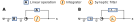
\includegraphics{media/chapters/02_modelling/02_03/nef_dynamics_diagram_ab.pdf}
	{\phantomsubcaption\label{fig:nef_dynamics_integral}}%
	{\phantomsubcaption\label{fig:nef_dynamics_synaptic}}%
	\caption[Integrator and synaptic filter realisations of an LTI system]{Integrator and synaptic filter realisations of an \LTI system. Orange circles depict temporal convolutions.
	\textbf{(A)} The standard \LTI system.
	\textbf{(B)} Using a low-pass filter instead of a perfect integrator.}
	\label{fig:nef_dynamics_ab}
\end{figure}

This principle is best explained considering linear time-invariant (\LTI) systems of the form
\begin{align*}
	\dot{\vec x}(t) &= \mat A \vec x(t) + \mat B \vec u(t) \,,
\end{align*}
where $\mat A \in \mathbb{R}^{\Ndim \times \Ndim}$ is the feedback matrix, and $\mat B \in \mathbb{R}^{\Ndim \times \Ndim'}$ is the input matrix.
Integration yields
\begin{align}
	\vec x(t)
	&=
		\int_0^t \dot{\vec x}(\tau) \,\mathrm{d}\tau + \vec x_0
	=
		\int_0^t \mat A \vec x(\tau) + \mat B \vec u(\tau) \,\mathrm{d}\tau + \vec x_0 \,,
	\label{eqn:lti_integral_equation}
\end{align}
where $\vec x_0$ is the initial state.
Hence, and as illustrated in \Cref{fig:nef_dynamics_integral}, if we have access to an integrator as a computational primitive, we can easily evaluate dynamical systems of this form.
%In practice, such integral equations can be evaluated using some numerical integration method, the simplest (but least powerful) being Euler integration \citep[cf.][Chapter~17]{press2007numerical}.

Unfortunately, biological neural networks do not contain \enquote{perfect} integrators.
Instead, they need to rely on \enquote{leaky} integrators, such as low-pass filters.
It is easy to see why a low-pass filter is a leaky integrator.
The impulse response of an integrator is a step function (i.e., zero for $t < 0$, one for $t \geq 0$).
Similarly, the impulse response $h(t)$ of a first-order low-pass filter jumps to non-zero value at $t = 0$, but in contrast to the integrator, quickly decays (\Cref{fig:first_order_low_pass}).
The key idea of the dynamics principle is to compensate for this \enquote{forgetfulness}.
That is, we change the desired dynamical system to account for leaky integration (\Cref{fig:nef_dynamics_synaptic}).

Despite the name, the \enquote{leaky integrator} dynamics of the \LIF neuron itself are of little use.
The neuron resets its state with every output spike, loosing all the integrated information.
Fortunately, the low-pass filter dynamics of synapses are decoupled from the neural superthreshold dynamics.
Moreover, as explained by
\citet[Chapter~8 \& Appendix~F.1]{eliasmith2003neural},
it is not unreasonable to assume that the synaptic filter dominates the overall neural dynamics.
In other words, dynamics mainly stem from the synaptic filter $h(t)$.
We revisit this assumption in \Cref{sec:nef_limitations} below.

We can easily derive a system that compensates for the low-pass filter dynamics using the Laplace transform.
Assume that both the feedback and the input passes through the same first-order low-pass filter with time-constant $\tau$.
Treating both the integral in \cref{eqn:lti_integral_equation} and the low-pass filter as convolutions with their respective impulse response, we have
\begin{align}
	X(s) &= \frac{1}{s} \bigl( \mat A X(s) + \mat B U(s) \bigr) & \text{and} \quad\quad X(s) &= \frac{1}{1 + \tau s} \bigl( \mat A' X(s) + \mat B' U(s) \bigr) \,.
	\label{eqn:original_vs_modified_lti}
\end{align}
Rearranging the second equation and comparing coefficients to the first equation we get
\begin{align}
	X(s) &= \frac{1}{s} \Big( \frac{\mat A' - \mat I}{\tau} X(s) + \frac{\mat B'}{\tau} U(s) \Big) &
	\leadsto \quad \quad \mat A' &= \tau \mat A + \mat I \,, &
	\mat B' &= \tau \mat B \,.
	\label{eqn:nef_transform_a_b}
\end{align}
For arbitrary dynamics $f(\vec x, \vec u, t)$ we similarly obtain $f'(\vec x, \vec u, t) = \tau f(\vec x, \vec u, t) + \vec x$ \citep[Appendix~B.3]{eliasmith2013how}.
In other words, to compensate for low-pass filter dynamics, we scale the dynamics by $\tau$ and feed back $\vec x$ to \enquote{remind} the system of its current state.

\begin{figure}
	\centering
	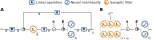
\includegraphics{media/chapters/02_modelling/02_03/nef_dynamics_diagram_c.pdf}%
	{\phantomsubcaption\label{fig:nef_dynamics_neurons_a}}%
	{\phantomsubcaption\label{fig:nef_dynamics_neurons_b}}%
	\caption[Synaptic filters and LTI systems in NEF networks]{Synaptic filters and \LTI systems in \NEF networks.
	\textbf{(A)} \NEF realisation of an \LTI system. Homogeneous synaptic filters are modelled as $d$ filters placed before the encoder.
	\textbf{(B)} Technically, each of the $n \times m$ synaptic connections between a pre- and a post-population has its own synaptic filter. When scaled appropriately, the resulting filter matrix replaces the synaptic weights; however, this has drastically higher computational costs than placing $d$ filters ahead of the encoder.}
	\label{fig:nef_dynamics_neurons}
\end{figure}

Using the representation and transformation principles, we can turn the block-diagram in \Cref{fig:nef_dynamics_synaptic} into a spiking neural network.
This is schematically depicted in \Cref{fig:nef_dynamics_neurons_a}.
The decoded state $\vec{\hat x}$ and the input $\vec u$ are passed through compensated \LTI matrices $\mat A'$ and $\mat B'$, summed, and fed into the synaptic filters.
We provided an example of this in \Cref{fig:nef_overview}.

Of course, as before, the network can, due to linearity, be expanded into biologically plausible synaptic weights and arrays of synaptic filters (\Cref{fig:nef_dynamics_neurons_b}).
Function decoders $\mat D^f$ can be used to support arbitrary nonlinear dynamics, and not just \LTI systems.

\subsection{Some Limitations of the Neural Engineering Framework}
\label{sec:nef_limitations}

To date, the Neural Engineering Framework has seen considerable use in the scientific community (cf.~\Cref{app:nef_literature}).
Nevertheless, the \NEF has a series of shortcomings that limit the biological plausibility of the generated networks, the number of constraints exposed to modellers, and how well resources available on some neuromorphic hardware platforms are utilised.
Resolving these issues could make the \NEF more appealing to a wider group of researchers and contribute to ongoing efforts in cognitive science and neuromorphic computing.

Of course, the following list of limitations is by no means complete.
To the contrary.
One can quite effortlessly identify areas of neuroscience that are not reflected in the \NEF at all---for example nervous system development, or networks of glial cells.
However, as we implied in the beginning this chapter, we think that, as of now, there is too little consensus on these topics to account for them in a general-purpose modelling tool.

Overall, while it is tempting to incorporate as much biological detail as possible into \NEF networks, this is misguided if merely done as an end in itself.
Remember that our goal is to bridge low-level mechanism and high-level function.
This distinguishes \NEF models from \enquote{bottom-up} approaches, that develop mechanistically detailed models of brain circuits, with the hope that the final system---if truthfully describing biology---exhibits some interesting function \citep[cf.][]{komer2016unified}.
We think that, optimally, extensions to the \NEF should expose new low-level detail as a \enquote{computational resource} that can be systematically exploited for high-level function.
At the very least, extensions should expose additional constraints that provide modellers with an opportunity to explore the impact of individual aspects of neurobiological mechanism on high-level function \citep[e.g.,][]{duggins2017incorporating}.
% TODO: Cite Pete's paper when published

%The two main extensions to the NEF we discuss in this thesis---nonlinear dendritic interactions and temporal tuning---fall into the first category, whereas the other extensions provide additional modelling constraints.

\subsubsection{Limitation 1: Current-based synapses}
In our discussion of Principle 2 (\Cref{sec:nef_transformation}), we implicitly assumed that neurons use current-based synapses (cf.~\Cref{sec:simplified_neuron_models}).
As expressed in \cref{eqn:nef_weight_vector}, we model the current injected into the post-neuron as linearly depending on the pre-population activities.
However, as we discussed in \Cref{sec:synaptic_transmission}, synaptic transmission is better modelled in terms of \emph{conductances}, and not currents.
As noted by \citet[Section~2.1.2, p.~35]{eliasmith2003neural}, accounting for conductances adds another layer of nonlinearity to the neuron.
While such nonlinearities have been analysed in the context of the \NEF by \citet[Chapter~4]{tripp2009search} as well as \citet{bobier2014unifying}, this prior work does not propose a systematic method for exploiting synaptic nonlinearities for computation.

Adapting the \NEF to support nonlinear conductance-based synapses would increase compatibility with neuromorphic hardware platforms emulating conductance-based neurons (e.g.,~BrainScaleS; \cite{schemmel2010waferscale}) and allow modellers to more easily constrain models according to neurophysiological parameters, such as synaptic reversal potentials.
Furthermore, individual synapse types (e.g.,~excitatory and inhibitory) act as independent input channels to a neuron.
As we discuss in the next chapter, these input channels interact nonlinearly in the case of multi-compartment neurons, increasing the class of functions that can be approximated using the same number of neurons.


\subsubsection{Limitation 2: Bias currents}
A minor (as we will see) limitation is the assumption that each neuron possess an intrinsic bias current $\beta_i$ (eq.~\ref{eqn:encoding}).
This current is necessary to ensure diverse tuning.
For example, some neurons are active even if no input is present (\enquote{spontaneous} or \enquote{background} activity).
This can be modelled using positive bias currents.

\Citet[Chapter~2; p.~35]{eliasmith2003neural} interpret the bias current as a \enquote{constant input current from the rest of the nervous system}.
While reasonable, this assumption cannot be strictly true.
The mean firing rate of individual populations varies sigificantly over time \citep{okun2012population}; it is not immediately clear how these variations would support constant $\beta_i$.
Hence, an explicit translation of pre-activities into a bias current $\beta_i$ using synaptic connectivity may be preferable.
Depending on the pre-population tuning, this can affect high-level function.


\begin{figure}
	\includegraphics{media/chapters/02_modelling/02_03/granule_jbias_distribution.pdf}%
	{\phantomsubcaption\label{fig:jbias_a}}%
	{\phantomsubcaption\label{fig:jbias_b}}%
	{\phantomsubcaption\label{fig:jbias_c}}%
	{\phantomsubcaption\label{fig:jbias_d}}%
	{\phantomsubcaption\label{fig:jbias_e}}%
	{\phantomsubcaption\label{fig:jbias_f}}
	\caption[Neuron parameter variability only accounts for small bias currents]{Neuron parameter variability only accounts for small bias currents.
	\textbf{(A, B)} Standard \NEF tuning curves and corresponding bias current distribution.
	\textbf{(C)} Empirical data on resting potential $v_\mathrm{rest}$ variations in cerebellar granule cells from \citet[Figure~1b]{chadderton2004integration} with a Gaussian fit.
	\textbf{(D)} Noisy \LIF neuron response curves for resting potentials samples from the empirical distribution. Colours indicated in \emph{(C)}. Other \LIF parameters fit to empirical data at $v_\mathrm{rest} = \SI{-64}{\milli\volt}$ (black crosses; cf.~Figure~1g in Chadderton et al.). Input currents $J$ are subject to Gaussian noise ($\sigma = \SI{10}{\pico\ampere}$). \textbf{(E)} Histogram of bias currents $\beta_i$ having the same average effect as varying $v_\mathrm{rest}$.
	\textbf{(F)}~Tuning curves that can be realised using these bias currents for the target maximum rates.
	Unfortunately, the empirically observed parameters do not result in tuning curve distributions assumed by the \NEF \emph{(A)}.}
	\label{fig:granule_jbias_distribution}
	\vspace*{-0.5em}
\end{figure}

Furthermore, and directly related to Limitation~1, pre-synaptic activity affects synaptic \emph{conductances} and does not directly induce \emph{currents}.
This is particularly problematic since tuning curves with uniform $x$-intercepts tend to require large \emph{negative} bias currents (\Cref{fig:jbias_a,fig:jbias_b}).
It is unclear how such currents should be generated, particularly since the inhibitory synaptic reversal potential $E_\mathrm{I}$ is close to the resting potential $v_\mathrm{rest}$.
Natural neuron parameter variations are insufficient to explain this discrepancy (\Cref{fig:jbias_c,fig:jbias_d,fig:jbias_e,fig:jbias_f}).

\begin{figure}
	\includegraphics{media/chapters/02_modelling/02_03/constrained_weight_matrices.pdf}
	{\phantomsubcaption\label{fig:sparsity_and_dales_principle_a}}%
	{\phantomsubcaption\label{fig:sparsity_and_dales_principle_b}}%
	{\phantomsubcaption\label{fig:sparsity_and_dales_principle_c}}%
	\caption[Constrained connectivity and Dale's principle]{Constrained connectivity and Dale's principle. \emph{Top:} Weight matrix $\mat W$ and (if applicable) factorisation into $\mat E, \mat D$. \emph{Bottom:} Weight histogram relative to the $95$-percentile $P_{95}$. Red indicates inhibitory, blue to excitatory weights. \textbf{(A)}~Typical \NEF weight matrices are dense.
	\textbf{(B)}~$L_1$-regularisation of decoders $\mat D$ increases sparseness, but does so in an uncontrolled manner. Note that $\mat D$ is (relatively speaking) sparser than $\mat W$.
	\textbf{(C)}~Dale's principle imposes an excitatory/inhibitory split on $\mat W$.
	This is difficult when factorising $\mat W$, but one can solve for $\mat W$ directly using nonnegative least-squares (\NNLS).
	}
	\label{fig:sparsity_and_dales_principle}
\end{figure}

\subsubsection{Limitation 3: Constrained connectivity and Dale's principle}
\NEF weight matrices $\mat W = \mat E \mat D$ are typically dense.
That is, they contain few zeros, implying all-to-all connectivity between neurons (\Cref{fig:sparsity_and_dales_principle_a}).
However, in biology, connectivity in the brain can be quite sparse.
For example, as detailed by \citet[Chapter~20]{braitenberg1998cortex}, the likelihood of two neighbouring cortical cells to be connected is less than $90\%$. Similarly, connectivity between Golgi and Granule cells in the cerebellum is highly constrained (cf.~Chapter~5).
% TODO: Add reference to Chapter 5
It may be desirable to give modellers the opportunity to account for these statistics.

A common way to enforce sparsity is to use $L_1$, or \enquote{lasso}, regularisation instead of the $L_2$ regularisation proposed in \cref{eqn:lstsq_loss_identity,eqn:lstsq_loss_f} \citep[Chapter~6]{boyd2004convex}.
However, solving for sparse decoders $\mat D$ in this way has two issues.
First, this process is uncontrolled---na\"ive $L_1$ regularisation does not take biological constraints into account.
Second, for $\Ndim \gg 1$, orthogonality between the encoders and decoders determines sparsity, and not just the sparsity of $\mat D$ (\Cref{fig:sparsity_and_dales_principle_b}).
Both issues mandate more complex regularisation terms.

Another form of constrained connectivity is to account for Dale's principle.
As we discussed before in \Cref{sec:synaptic_transmission}, individual neurons typically act either exclusively excitatorily or inhibitorily. Empirical data suggest that, depending on the modeled brain region, excitatory cells outnumber inhibitory cells by a factor between two and four~\citep{hendry1981sizes,gabbott1986quantitative}.
This imposes a certain structure onto the weight matrix (\Cref{fig:sparsity_and_dales_principle_c}).

\begin{figure}
	\centering
	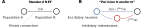
\includegraphics{media/chapters/02_modelling/02_03/parisien_transform.pdf}
	\caption[Illustration of the \enquote{Parisien transform}]{Illustration of the \enquote{Parisien transform}. This transformation accounts for Dale's principle by splitting standard \NEF connections, as depicted in \textbf{(A)}, into an excitatory and inhibitory path \textbf{(B)}.}
	\label{fig:parisien_transform}
\end{figure}

\Citet[Section~6.4]{eliasmith2003neural} propose a method to account for Dale's principle later refined by \citet{parisien2008solving}.
The basic idea of this \enquote{Parisien transform} is to add a specially crafted \enquote{bias function} to the function computed in the excitatory connection.
This bias function ensures that all connection weights are positive.
An inhibitory inter-neuron population is then added to the network and connected in parallel to the excitatory connection to subtract the superfluous current induced by the bias function (\Cref{fig:parisien_transform}).

While mathematically clever, the Parisien transform changes the network structure by adding an inhibitory interneuron population.
Although interneurons are indeed common in brain networks, the connectivity patterns resulting from the Parisien transform may not be desirable.
For example, as we discuss in Chapter~5, Golgi cells are recurrent inhibitory interneurons between granule cells.
However, there are no excitatory recurrent connections between granule cells, as assumed by the Parisien transform.
In the next chapter, we discuss an approach to accounting for Dale's principle that is independent of the network structure.

\subsubsection{Limitation~4: Temporal tuning and neural dynamics}
The dynamics principle derived in \Cref{sec:nef_dynamics} was based on two assumptions.
First, synaptic dynamics dominate neural dynamics.
Second, synaptic filters are homogeneous first-order low-pass filters in both the input and recurrent connection.
While reasonable, these modelling assumptions are, as so often, only coarse approximations of biology.

\begin{figure}[t]
	\includegraphics{media/chapters/02_modelling/02_03/firing_rate_neural_dynamics.pdf}
	\caption[Neural dynamics for different maximum firing rates]{Neural dynamics for different maximum firing rates $a_\mathrm{max}$. A \SI{100}{\second} band-limited white-noise signal $u(t)$ with a band-width of \SI{100}{\hertz} is fed through an \NEF population with uniform $x$-intercepts.
	The transfer function is determined from the decoded $\hat u(t)$ using the method described in \citet[Section~4.3.3]{eliasmith2003neural}.
	We ensure a constant amount of spike noise by setting the number of neurons in the population to $100\,000 / a_\mathrm{max}$. \emph{Top:} Linear transfer function for different maximum rates $a_\mathrm{max}$. \emph{Bottom:} Slice through the transfer functions at the indicated locations.
	\textbf{(A)} Data for a spiking rectified linear unit (\ReLU), a $\Delta\Sigma$-modulator with a rectified input current. This kind of neuron exhibits no significant dynamics of its own, independent of the firing rate. \textbf{(B)} Transfer function for the \LIF neuron. For small firing rates, the neuron acts as a low-pass with a relatively moderate attenuation of about \SI{-5}{\deci\bel}. For firing rates of about \SI{200}{\hertz}, the neuron acts as a pass-through. \textbf{(C)} While similar to the \LIF neuron, the \ALIF
	acts as a very narrow low-pass filter when driven at a maximum firing rate of about \SI{20}{\hertz}. The location of this \enquote{trough} depends on the adaptation time-constant.}
	\label{fig:neural_dynamics_firing_rates}
\end{figure}

The assumption that synaptic dynamics dominate the overall dynamics of a neuron is a good approximation of the behaviour of simple neuron models operating at high firing-rates.
However, for smaller firing rates, the neural dynamics can have a significant impact on the overall system dynamics.
For example, for maximum firing rates below about $\SI{50}{\per\second}$, the sub-threshold low-pass dynamics of the \LIF neuron begin to have a moderate effect on the neural dynamics.
This is depicted in \Cref{fig:neural_dynamics_firing_rates}.

While these rate-dependent effects are relatively small, more complex neuron models possess strong intrinsic dynamics.
For example, the adaptive \LIF (\ALIF) neuron model \citep{camera2004minimal} accounts for firing rate adaptation; that is, each output spike increases the current required to evoke another output spike.
This can be modelled as an inhibitory current resulting from low-pass filtering the neuron's output spike train.
As demonstrated by \citet[Chapter~7]{tripp2009search}, the internal dynamics of the \ALIF neuron model can, under certain circumstances, be exploited to implement arbitrary dynamics using a variant of the equations derived for the \NEF dynamics principle.

The second assumption, namely that synaptic filters are homogeneous, is likely violated if a neuron possesses multiple receptor types.
As we saw in \Cref{sec:synaptic_transmission}, the synaptic time-constant can vary significantly between (and even within) individual receptor types.
We also saw that synaptic transmission is better modelled by higher-order filters.
\Citet{voelker2018improving} discuss methods to generalise the dynamics principle to arbitrary synaptic filters; however, these methods require access to the input signal differentials.

In \Cref{chp:temporal_tuning}, we suggest the concept of \enquote{temporal tuning curves} to---at least partially---account for these issues.
Temporal tuning curves are a direct extension of standard \NEF tuning curves, and are inspired by the concept of temporal receptive fields.
In essence, we treat both synaptic and neural dynamics as temporal resources that can be harnessed to approximate a desired temporal tuning by solving a simple least-squares problem.
This naturally extends the \NEF and, to an extent, unifies the approaches described by Tripp and Voelker systematically.

